
\addtocounter{part}{1}

\part[II]{Microscopic Processes}
\begin{frame}
  \partpage
  \tableofcontents[part=2]
\end{frame}



%\begin{frame}\frametitle{Microscopic processes in the ISM}
%
%%\begin{minipage}[t]{13cm}
%%\end{minipage}
%
%\vspace{-1cm}
%\begin{enumerate}
% \item Thermal equilibrium \label{item:Teq}
% \begin{enumerate} 
%  \item  Cooling of the  ISM - collisional excitation \label{item:Teq_cool}
%  \begin{enumerate} 
%    \item ionic excitation \label{item:Teq_cool_ion}
%%    \begin{enumerate} 
%%      \item cooling of H\,{\sc ii} regions \label{item:Teq_cool_hii}
%%      \item cooling of the neutral ISM \label{item:Teq_cool_neutral}
%%    \end{enumerate}
%    \item molecular excitation - CO \& H$_2$ \label{item:Teq_cool_molecule}
%    \item summary: diatomic molecules \label{item:Teq_cool_molstruct}
%   \end{enumerate}
%  \item Cooling of the  ISM - radiative transitions \label{item:Teq_cool_rad}
%  \begin{enumerate}
%    \item  Interaction with electromagnetic radiation \label{item:Teq_cool_rad_H}
%    \item  Transition probabilities \label{item:Teq_cool_rad_prob}
%\end{enumerate}
%\item heating of the  ISM \label{item:Teq_heat}
%%\begin{enumerate}
%%\end{enumerate}
%\end{enumerate}
%\item Molecule formation \label{item:molec}
%\begin{enumerate} 
%\item \label{item:molec_grain} grain catalysis of the formation process of  H$_2$
%\item \label{item:molec_H3+}Molecule formation - the
%role of H$_3^+$.
%\item \label{item:molec_valid} Validation of the ion-molecule model.
%\end{enumerate}
%\item \label{item:fractio} Chemical Fractionation
%\end{enumerate}
%
%
%
%\end{frame}

\section{Thermal Equilibrium of the ISM}

 \begin{frame}\frametitle{Thermal Equilibrium of the ISM}



\centering

\[  \underbrace{n \frac{d}{dt} \left( \frac{3}{2} k T
  \right)}_{\mathrm{variation ~of ~ internal ~E.}} -
\underbrace{kT\frac{dn}{dt}}_{\mathrm{power}}
 = \overbrace{
\stackrel{\mathrm{cooling ~rate}}{\Gamma}  -
\stackrel{\mathrm{heating}}{\Lambda}}^{\mathrm{J~s^{-1}~cm^{-3}}}\]

\raggedright
In steady state, $dn/dt = dT/dt = 0$, so the temperature $T$
is determined by  $\Lambda(T)  = \Gamma(T) $.


\end{frame}

\subsection{Cooling of the ISM: detailed balance, critical density}


\begin{frame}\frametitle{Cooling of the ISM}


Radiative cooling (ref.  Dyson \& Williams, Chap. 3, Spitzer, Chap. 4 \&
6, Osterbrock, Chap. 3). \medskip


\centering
\begin{minipage}[t]{6cm}
\begin{eqnarray*}
 A + B  & \rightarrow &  A + B^{\star} \\
 B^{\star} & \rightarrow  & B + h\nu  
\end{eqnarray*}
\end{minipage} 
\hfill
\begin{minipage}[t]{19cm}
Requisites for a mechanism of radiative cooling
\begin{itemize}

\item frequent encounters, i.e. $A$ \& $B$ abundant
\item $E(B^{\star}) - E(B) \ls k T$. 
\item large rate of $B$ excitations:  high  `collision strength'
\item time scale for radiative decay of  $B^\star$ less than  $\tau_\mathrm{col}$ 
\item large escape probability of the output $h\nu$.
\end{itemize}
\end{minipage} 
\vfill


%\subsubsection{Detailed balance}

\end{frame} \begin{frame}\frametitle{Detailed balance: abundance of
    excited species}

\raggedright

In steady state, the density $n_j$ of species $B^\star$ in level $j$
is determined by an equation of detailed balance, which models systems
with a finite number of microscopic states:
\begin{eqnarray*}
\lefteqn{\sum_k    \left(    \left\{ \begin{array}{c}  n_\mathrm{e} \\
    n_\mathrm{H_2} \\  n_\mathrm{H_I} \end{array} \right\}    n_j
  \gamma_{jk} +  {n}_{j} B_{jk} J_\nu \right) + \sum_{k<j} \left( A_{jk} n_j  \right)   } \\   
& &     =    \sum_k \left(  n_k      \left\{ \begin{array}{c}  n_\mathrm{e} \\  n_\mathrm{H_2} \\  n_\mathrm{H_I} \end{array} \right\}  \gamma_{kj} + B_{kj} J_\nu n_k \right) + \sum_{k>j} \left( n_k A_{kj} \right),
\end{eqnarray*}
which we may also write using a  simplified notation: 
\[\sum_{i{\neq}j}
{n}_{j}{C}_{ji} + {n}_{j}{B}_{ji} U_{\nu_{ji}} +
\sum_{i<j}{n}_{j}{A}_{ji} = \sum_{i{\neq}j}{n}_{i}{C}_{ij} +  {n}_{i}{B}_{ji} U_{\nu_{ij}} + \sum_{i>j}{n}_{i}{A}_{ij}. 
\]

\vfill



%\end{frame} \begin{frame}\frametitle{\textcolor{red}{B$_1$} Enfr\'{\i}amento   del ISM  }
\end{frame} \begin{frame}\frametitle{Detailed balance: rate of collisonal excitation}

For any collision partner (i.e. either $\begin{array}{c}  n_\mathrm{e}
\\  n_\mathrm{H_2} \\  n_\mathrm{H_I} \end{array} $ ), the specific rate of
collisional excitations is

\[
\gamma_{jk} = \langle u \sigma_{jk}(u) \rangle = \frac{4}{\sqrt{\pi}} \left(\frac{m_r}{2kT} \right)^{3/2} \int_0^\infty du ~ u^3 \sigma_{jk}(u) \exp\left(  - \frac{m_r}{2kT} u^2 \right).
\]

 the specific rate (i.e. per pair of  particles, in units of
m$^{3}$~s$^{-1}$) of collisional de-excitations $\gamma_{kj}$ must be
related to $\gamma_{jk}$: in thermodynamic equilibrium any microscopic
process must be balanced by its inverse ({\em principle of detailed
balance}, otherwise the distribution functions would depend on $t$ and
there would be no equilibrium).

%\end{frame} \begin{frame}\frametitle{\textcolor{red}{B$_1$} Enfr\'{\i}amento   del ISM  }

\end{frame} \begin{frame}\frametitle{Milne relations}

In {\bf LTE} the rate of collisional excitations $j\rightarrow k$ with
relative velocity $\vec{u} \in [\vec{u},\vec{u}+d\vec{u}]$ must equal
the rate of de-excitations $k \rightarrow j$ in the corresponding
velocity range $\vec{v}$, \[
n^\mathrm{LTE}_j \begin{array}{c}  n_\mathrm{e} \\  n_\mathrm{H_2} \\  n_\mathrm{H_I} \end{array}  \sigma_{jk}(u) f(u)  u d\vec{u}  = 
n^\mathrm{LTE}_k \begin{array}{c}  n_\mathrm{e} \\  n_\mathrm{H_2} \\
n_\mathrm{H_I} \end{array}  \sigma_{kj}(v) f(v)  v d\vec{v}  , \]
with   $ f(u) =   \left(\frac{1}{\pi}\frac{m}{2kT} \right)^{3/2}
\exp\left(-\frac{m}{2kT} u^2 \right) $,  and~~ $ \frac{1}{2}m_r v^2 =
\frac{1}{2} m_r u^2 - E_{jk}$~\footnote{note threshold excitation energy},  
%\centering
\[\stackrel{\textcolor{red}{\mathrm{tarea}}} \Longrightarrow  ~~~~~  g_j u^2 \sigma_{jk}(u) = g_k v^2 \sigma_{kj}(v),~\text{or} \]
\[ C_{kj}=C_{jk} \frac{g_{j}}{g_{k}} e^{E_{jk}/kT} .\] 


%\subsubsection{Critical density}

\end{frame} \begin{frame}\frametitle{Critical density}

The {\em critical density} is defined as the density at which the rate
of collisonal de-excitations is equal to the rate of radiative
de-excitations:

\[\sum_{k<j} C_{kj} = \sum_{k<j} A_{jk} .\]

A good cooling mechanism is therefore one that involves abundant
species, an effective collision strength $\gs$1, a critical density
$n_\mathrm{crit} \gg n_\mathrm{e}$, and opticallly thin transport of
the output $h \nu_{jk}$.



\end{frame}
\subsection{Ionic \& atomic  cooling of the ISM}
 \begin{frame}\frametitle{Ionic  \& atomic  cooling of the ISM}

For ionic collisions, the cross-section of collisional excitation
highlights the Coulomb cross-section.
\[ \sigma_{jk}(E)=\frac{\pi a_{\circ}^{2}  \Omega_{jk}(E)}{E/E_{\circ}}, \]
where $E_{\circ}$ is ~1~Rydberg, $a_{\circ}$ is the Bohr radius, and
$\Omega_{jk}(E)$ (of order 1), is the {\em collision strength} as a
function of  kinetic energy $E$. Finally the rate of excitations $j
\rightarrow k$ (with units of s$^{-1}$) is (\textcolor{red}{tarea}),
\[
C_{jk}= \left\{ \begin{array}{c} n_\mathrm{e} \\ n_\mathrm{H_2} \\
n_\mathrm{H_I} \end{array} \right\} {\sqrt{\frac{2\pi}{kT}}}
{\left(\frac{h}{2\pi}\right)}^{2}
\frac{1}{m_r^{3/2}} \frac{\Gamma_{jk}}{g_{j}} e^{-E_{jk}/kT},
\] where  $\Gamma_{jk}$,  the   {\em  effective collision strength},
is the Maxwellian average of $\Omega(E)$.

%\end{frame} \begin{frame}\frametitle{\textcolor{red}{B$_1$} Enfr\'{\i}amento   del ISM  }

\end{frame} \begin{frame}\frametitle{Fine structure cooling in the IR}

In LS coupling energy levels are ordered according to the Hund rules
(Shu I Chap. 27):

\begin{itemize}
\item Higher S $\rightarrow$ lower energy
\item Higher L $\rightarrow$ lower energy
\item Higher J $\rightarrow$ higher energy if less than half-filled,
lower energy if more than half-filled
\end{itemize}

Spectroscopic notation in spin-orbit coupling (ver Shu
I,27):
\LARGE \\ \medskip
\( \mathrm{^{2S+1} L_J   } \) \normalsize, with degeneracy (2~J+1)

\textcolor{blue}{\bf Examples:} 
\begin{itemize}
\item  $[$Ar\,{\sc vi}$]$~4.52$\mu$m, $^2$P$_\frac{1}{2}\leftarrow ^2$P$_\frac{3}{2}$, Z=18
\item  $[$Al\,{\sc vi}$]$~3.65$\mu$m, $^3$P$_2\leftarrow ^3$P$_1$, Z=13
\end{itemize}


\end{frame} \begin{frame}\frametitle{Ar\,{\sc vi}  $^2$P$_\frac{3}{2}$
  population}

\begin{center}
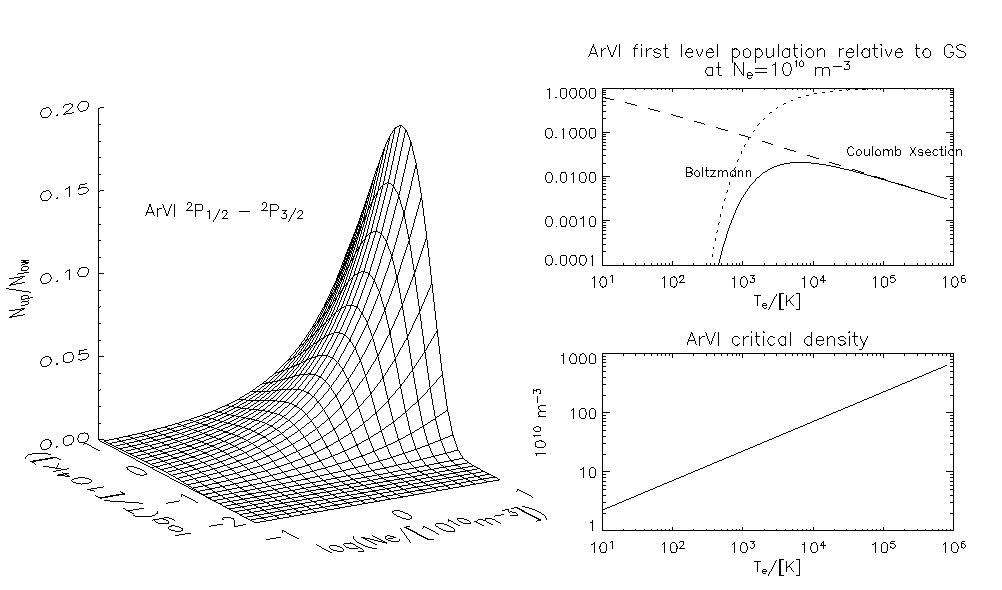
\includegraphics[width=\textwidth,height=!]{./B/ArVI_pop.pdf}
\end{center}

\end{frame} \begin{frame}\frametitle{ Ar\,{\sc vi}  $^2$P$_\frac{3}{2}$
  population}


\begin{center}
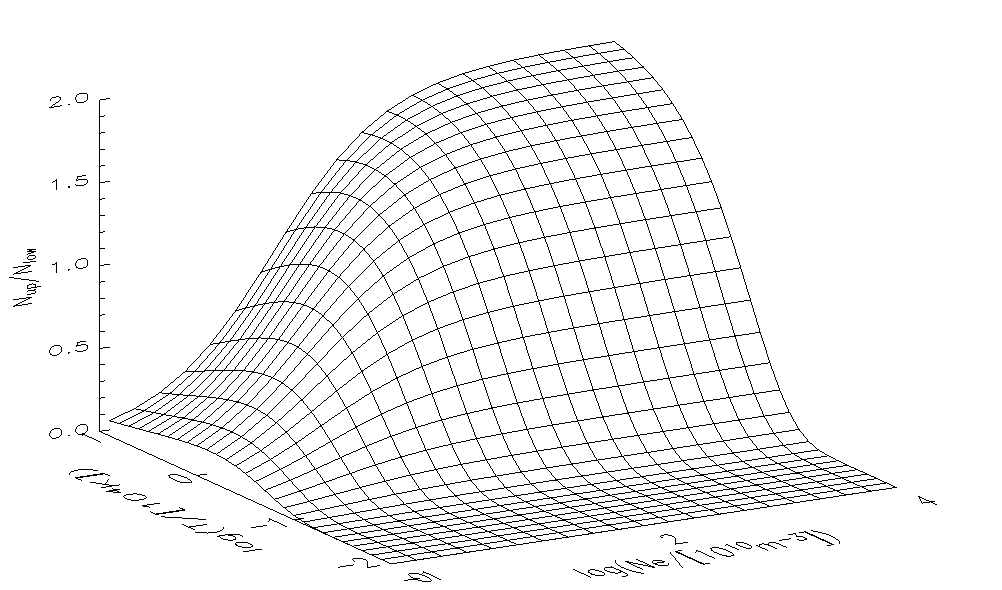
\includegraphics[width=\textwidth,height=!]{./B/ArVI_pop_xtd.pdf}
\end{center}

%%%%%%%%%%%%%%%%%%%%%%%%%%%%%%%%%%%%%%%%%%%%%%%%%%%%%%%%%%%%%%%%%%%%%%%%%%%
%%%%%%%%%%%%%%%%%%%%%%%%%%%%%%%%%%%%%%%%%%%%%%%%%%%%%%%%%%%%%%%%%%%%%%%%%%%
%%%%%%%%%%%%%%%%%%%%%%%%%%%%%%%%%%%%%%%%%%%%%%%%%%%%%%%%%%%%%%%%%%%%%%%%%%%

\end{frame} \begin{frame}\frametitle{Cooling of H\,{\sc ii} regions}
%\leftheader{B-\ref{item:Teq_cool_hii}:  Cooling of }

%\end{frame} \begin{frame}\frametitle{\textcolor{red}{B$_1$} Enfr\'{\i}amento  de regiones H\,{\sc ii} }

For gas in a steady state, where every ionization event is balanced by
a recombination event (case of a nebula photoionised by OB stars), the
cooling mechanisms are:


\begin{enumerate}

\item Recombination radiation (postponed to chapter on photoionised nebulae)
\item Continuum emission (free-free, bound-free):  $A + B   \rightarrow   A +
  B + h\nu $ (postponed to chapter on
  photoionised nebulae)

\item Collisionally excited line emission: 
$$\Lambda_{CE}= \sum_X \sum_i n(X,i) \sum_{j < i} A_{i,j}\, (E_i -
E_j)$$ e.g.
\begin{itemize}
\item   $[$O\,{\sc ii}$]\lambda\lambda$3726,3729 ~ $\mathrm{^4S_{3/2} \leftarrow ^2\!D_{3/2,5/2} } $.
%\item   $[$S\,{\sc iii}$]\lambda\lambda$9071,9533 ~ $\mathrm{^3P_{2,1} \leftarrow ^1D_{2} } $.
\item   $[$O\,{\sc iii}$]\lambda\lambda$4959,5007 ~ $\mathrm{^3P_{2,1} \leftarrow ^1D_{2} } $.
\end{itemize}

\end{enumerate}


\end{frame} \begin{frame}\frametitle{Cooling of H\,{\sc ii} regions: collisionally excited line radiation}

\begin{center}
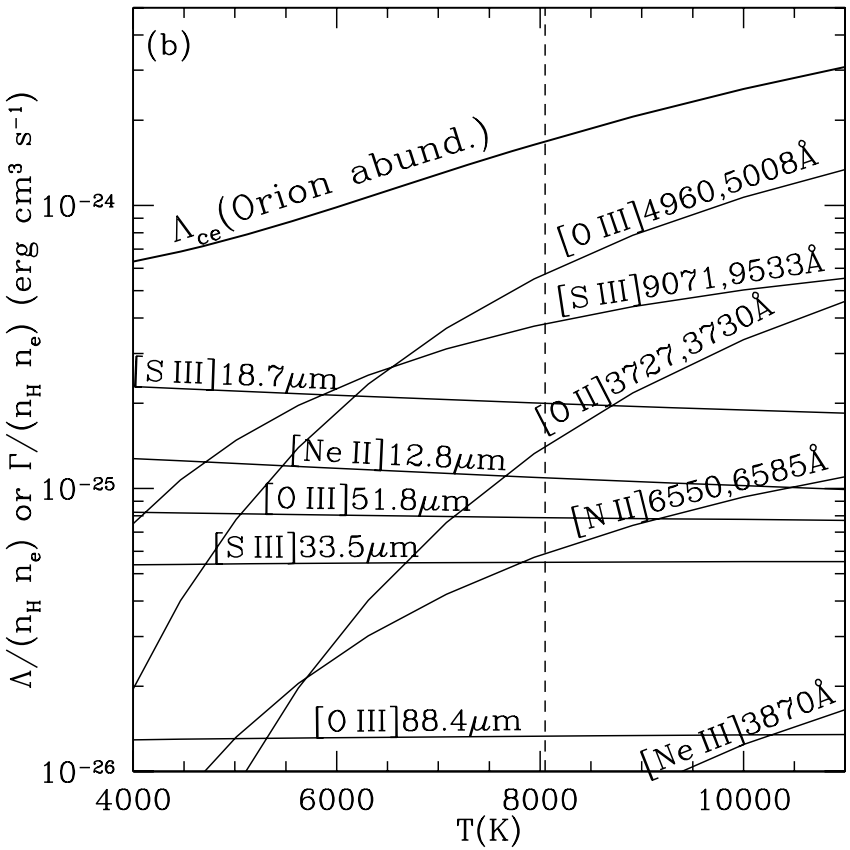
\includegraphics[width=0.8\textwidth,height=!]{./B/cooling_CE.png}
\end{center}

\end{frame} \begin{frame}\frametitle{Cooling of H\,{\sc ii} regions: collisionally excited line radiation}
$z \sim z_{\odot}$
\begin{center}
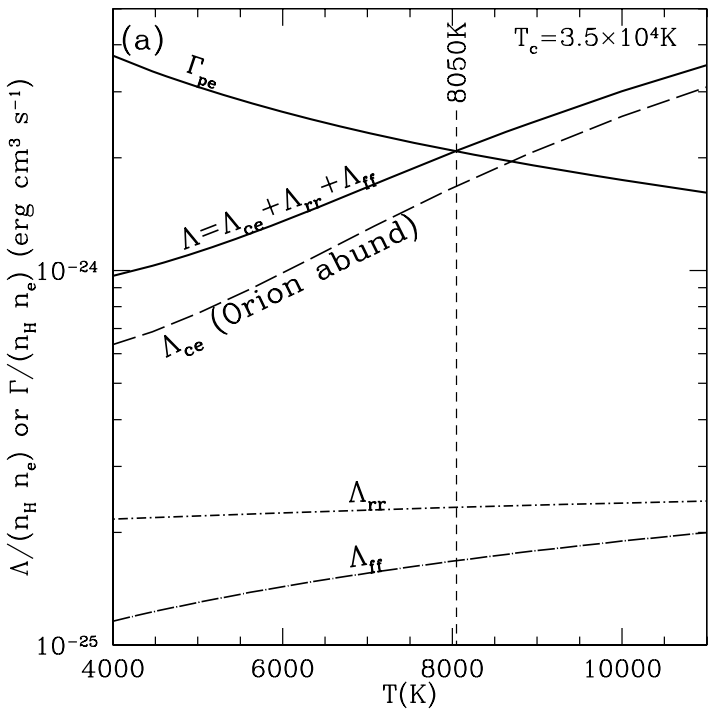
\includegraphics[width=0.8\textwidth,height=!]{./B/heating_cooling.png}
\end{center}


\end{frame} \begin{frame}\frametitle{Cooling of H\,{\sc ii} regions: collisionally excited line radiation}
$z \sim 0.1 z_{\odot}$
\begin{center}
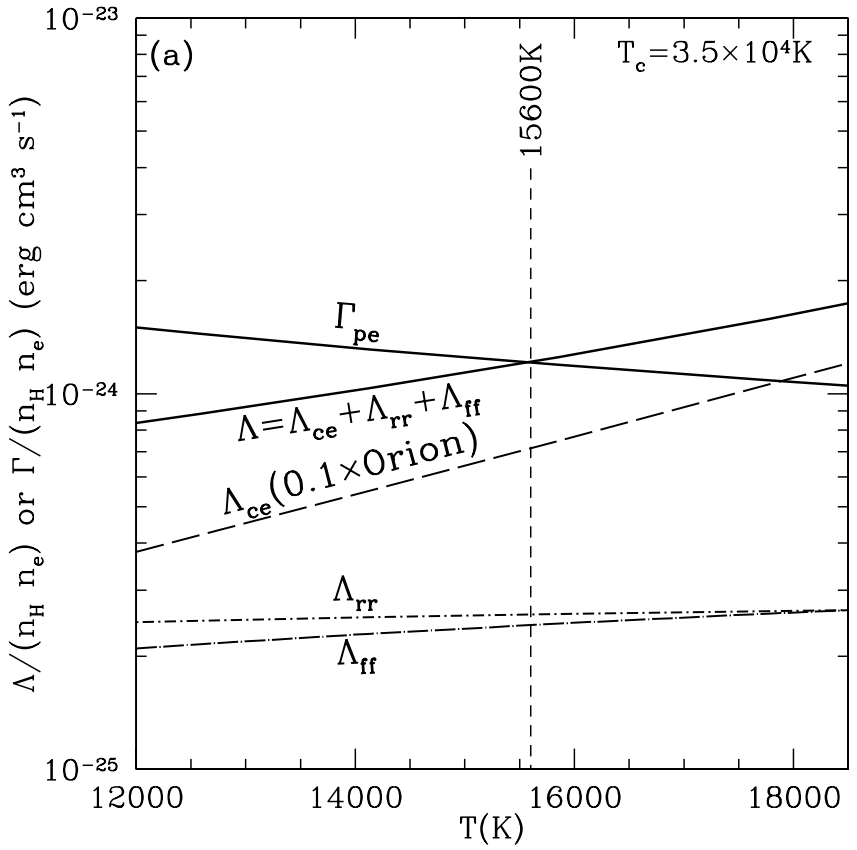
\includegraphics[width=0.8\textwidth,height=!]{./B/cooling_01.png}
\end{center}



\end{frame} \begin{frame}\frametitle{Cooling of H\,{\sc ii} regions: collisionally excited line radiation}
$z \sim 3 z_{\odot}$
\begin{center}
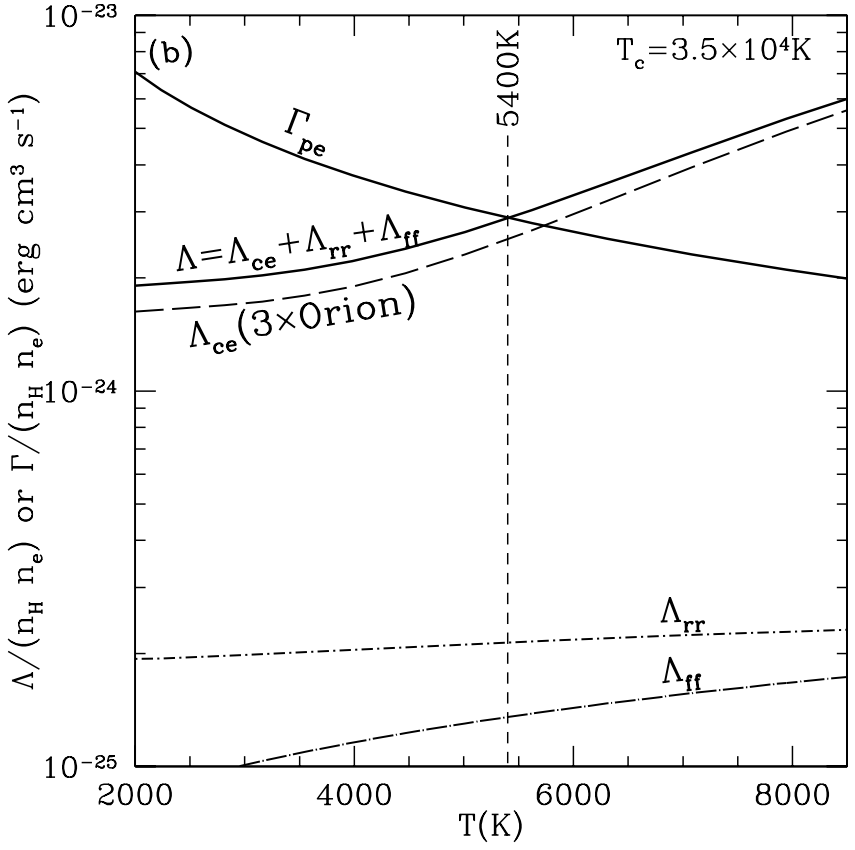
\includegraphics[width=0.8\textwidth,height=!]{./B/cooling_3x.png}
\end{center}






\end{frame} \begin{frame}\frametitle{Cooling of the neutral ISM}
%\end{frame} \begin{frame}\frametitle{\textcolor{red}{B$_1$} Enfr\'{\i}amento  del ISM neutro - \'atomos e {\em iones} }

%1576800.         [C II]      M1        2Po-2Po         1/2-3/2           .00 -       63.42
% 631850.         [O I]       M1         3P-3P            2-1             .00 -      158.26
%1455350.         [O I]       M1         3P-3P            1-0          158.26 -      226.98
% 348152.         [Si II]     M1        2Po-2Po         1/2-3/2           .00 -      287.23

Occurs through excitation of low-lying electronic states, fine
structure levels dominate.

Examples: Table~3.1 in Dyson \& Williams complemented by the list of
lines in {\tt http://www.pa.uky.edu/$\sim$peter/atomic/}

\begin{center}
\begin{tabular} {lll}
Transition   &    collision partner &  $\Delta E / k$ \\   \hline 
$[$C\,{\sc i}$]$~$\lambda$157.7\,$\mu$m ~ $\mathrm{^2P_{1/2} \leftarrow ^2P_{3/2} } $    & H,e,H$_2$  &   92~K \\
$[$Si\,{\sc ii}$]$~$\lambda$34.8\,$\mu$m ~ $\mathrm{^2P_{1/2} \leftarrow ^2P_{3/2} } $    & e  &   92~K \\
$[$O\,{\sc i}$]$~$\lambda$63.2\,$\mu$m ~ $\mathrm{^3P_{1} \leftarrow ^3P_{2} } $    & H,e  &   228~K \\
$[$O\,{\sc i}$]$~$\lambda$145.5\,$\mu$m ~ $\mathrm{^3P_{0} \leftarrow ^3P_{2} } $    & H,e  &   326~K \\
\end{tabular}
\end{center}




\end{frame} 

%

\begin{frame}\frametitle{Molecular excitation - CO \& H$_2$}

%\end{frame} \begin{frame}\frametitle{\textcolor{red}{B$_1$} Enfr\'{\i}amento  del ISM neutro - H$_2$ }

%1576800.         [C II]      M1        2Po-2Po         1/2-3/2           .00 -       63.42
% 631850.         [O I]       M1         3P-3P            2-1             .00 -      158.26
%1455350.         [O I]       M1         3P-3P            1-0          158.26 -      226.98
% 348152.         [Si II]     M1        2Po-2Po         1/2-3/2           .00 -      287.23

%Van Dishoeck, 2004, ARA\&A, 42, 119

{\em ISO} observations (Van Dishoeck, 2004, ARA\&A, 42, 119)
suggest that the contribution from H$_2$ cooling is more important
than estimates based on {\em IRAS} data: H$_2$ is among the brightest
emission lines in molecular clouds exposed to UV radiation, as for
instance in Orion~KL (note prominent dust continuuum):


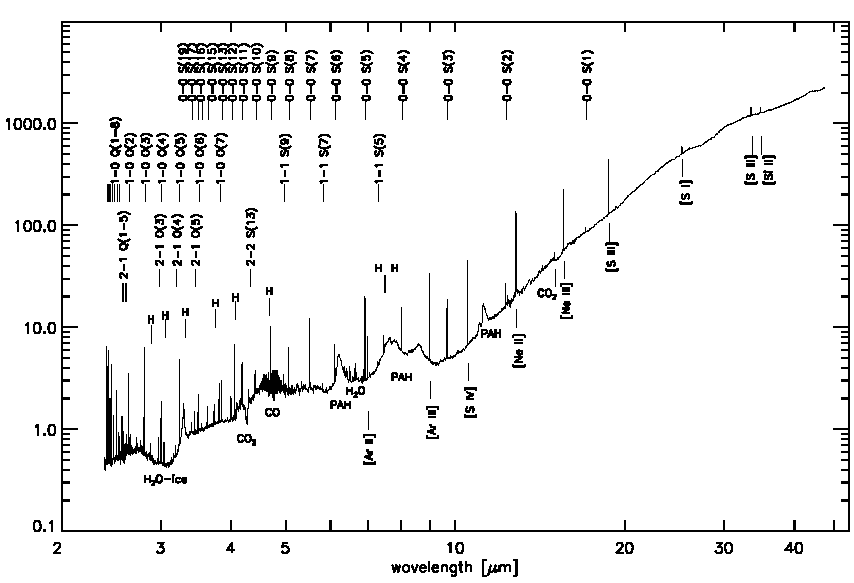
\includegraphics[width=0.8\textwidth,height=!]{./B/dishoeck_fig3.pdf}

\end{frame} \begin{frame}\frametitle{fluorescent H$_2$: not a gas coolant}

The rotational excitation of the ground vibrational state of H$_2$ is
usually collisional (i.e. thermal), while higher vibrational states are excited by fluorescence (hence not a cooling process). 

\medskip

$\Rightarrow$ near-IR rovib H$_2$ is usually fluorescent, so not a
coolant (except some of the lower-level rovib lines, in shocked regions). 

\vfill

\end{frame} \begin{frame}\frametitle{Dust continuum: not a gas coolant}

The most luminous spectral component in the molecular ISM is the
mid-IR to far-IR continuum, due to dust. Dust is responsible for
transporting the UV radiation of the exciting stars, but is not always
coupled to the molecular gas. Collisions are efficient dust heating
sources in the denser media only, such as dense SNRs or dense
circumstellar disks.

%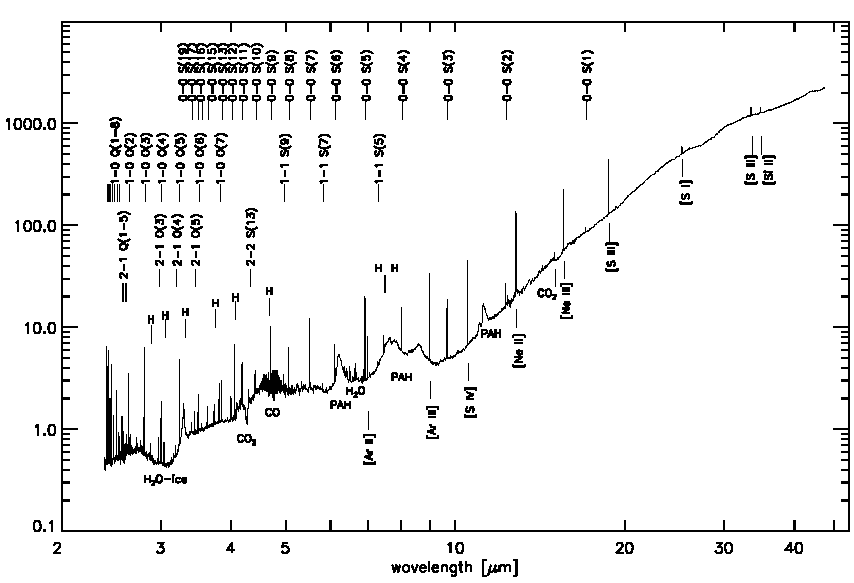
\includegraphics[width=0.7\textwidth,height=!]{./B/dishoeck_fig3.pdf}
\centering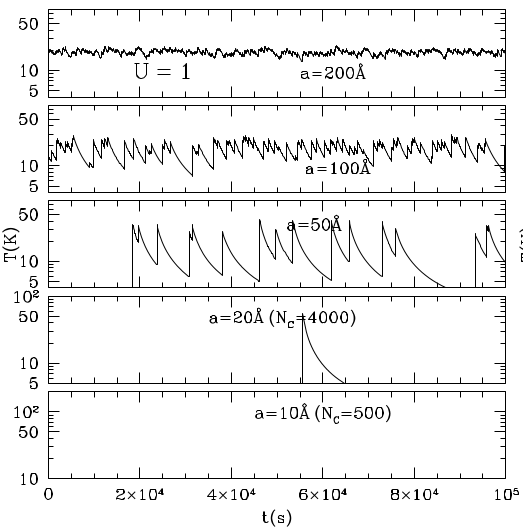
\includegraphics[width=0.6\textwidth,height=!]{./B/grain_temp.png}

\end{frame} \begin{frame}\frametitle{CO rotational-line cooling}
%\begin{minipage}{12.5cm}
%The main cooling agents for cold molecular clouds are low-level
%rotational transitions of CO in the sub-mm. (Figure 2.11 from Tielens
%2005).
%\end{minipage}
%\hfill
%\begin{minipage}{13cm}
%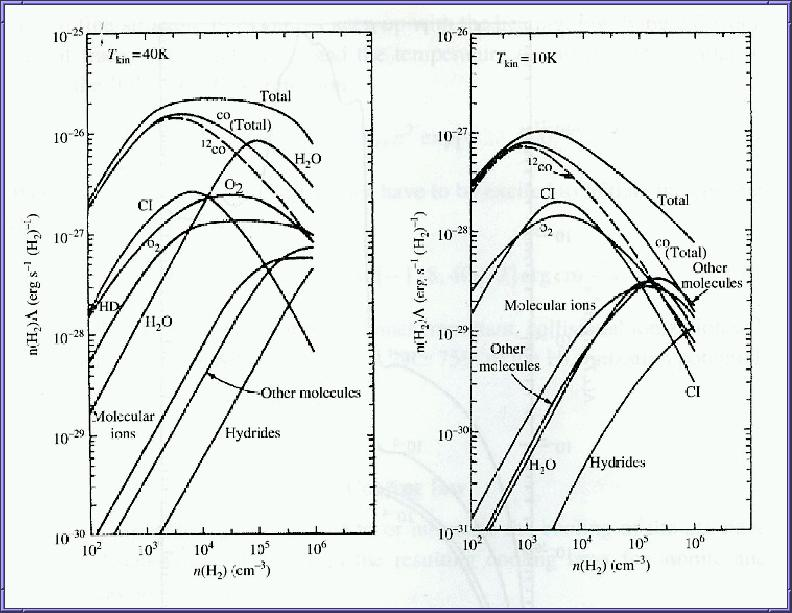
\includegraphics[width=13cm,height=!]{./B/CO_cooling_Tielens.jpg}
%\end{minipage}

The main cooling agents for cold molecular clouds are low-level
rotational transitions of CO in the sub-mm. (Figure 2.11 from Tielens
2005).
\begin{center}
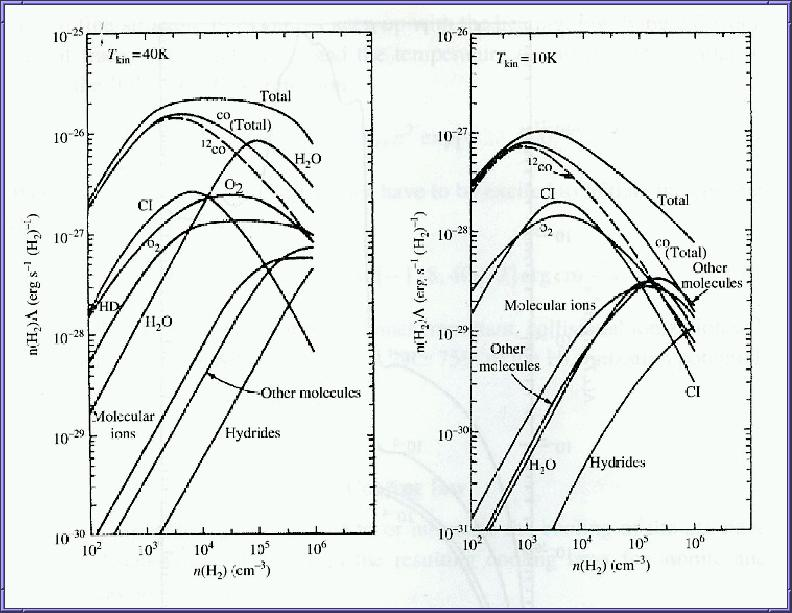
\includegraphics[width=0.8\textwidth,height=!]{./B/CO_cooling_Tielens.jpg}
\end{center}




\end{frame} 


%\subsubsection{Molecular structure}
\subsection{Molecular excitation \& molecular structure}
\begin{frame}\frametitle{Summary: diatomic molecules}

In the Born-Oppenheimer approximation the Hamiltonian for a diatomic
molecule AB separates, $H = H_\mathrm{AB} + H_\mathrm{el} $, where
$H_\mathrm{AB}$ represents the kinetic energy of the nuclei, and
$H_\mathrm{el}$ all the rest. It is also customary to factorize $\phi =
\phi_\mathrm{el}
\phi_\mathrm{AB}$ and obtain  \footnote{provided additional
approximations according to Messiah, Vol. 2, XVIII.64 (p791), but
exactly according to Shu I, 28. Probably valid only for processes
slower than a rotation period.}:
\[H_\mathrm{el}  \phi_\mathrm{el} = E_\mathrm{el}(R)~  \phi_\mathrm{el}, \] 
\[H_\mathrm{AB}  \phi_\mathrm{AB} +  E_\mathrm{el}(R)~ \phi_\mathrm{AB} = E~ \phi_\mathrm{AB}, \] 
and using the centre of mass coordinates, $\phi_\mathrm{AB} =
\phi_\mathrm{trans}(\vec{X}_\mathrm{CM}) \phi_\mathrm{intern}(\vec{R})
$,
\[ -\frac{\hbar^2}{2M} \nabla^2_\mathrm{CM} \phi_\mathrm{trans}  = E_\mathrm{trans} ~\phi_\mathrm{trans} \]
\[ -\frac{\hbar^2}{2\mu} \nabla^2_{\vec{R}} \phi_\mathrm{intern} + E_\mathrm{el}(R) ~\phi_\mathrm{intern}  = E_\mathrm{intern} ~\phi_\mathrm{intern},\]
with $E=E_\mathrm{intern}+E_\mathrm{trans}$.
\end{frame} \begin{frame}\frametitle{}
The Laplacian in spherical coordinates,
\[ \nabla^2_{\vec{R}} = \frac{1}{R^2} \left[ \frac{\partial}{\partial R} \left( R^2  \frac{\partial}{\partial R}  \right) - \frac{L^2}{\hbar^2} \right], \]
inspires the decomposition of the wave function for the internal
degrees of freedom in spherical armonics,
\[\phi_\mathrm{intern}(\vec{R}) = \frac{1}{R} Z_\mathrm{vib}(R) Y_{Jm}(\theta,\varphi), \]
The 1-D equation for $Z_\mathrm{vib}(R)$ is a function of
$E_\mathrm{el}(R)$, the energy eigenvalue of the electronic wave function:
\[-\frac{\hbar^2}{2\mu} \frac{d^2\,Z_\mathrm{vib}}{dR^2} +
E_\mathrm{el}(R)  Z_\mathrm{vib} = \left[ E_\mathrm{intern}  - \frac{
    J (J + 1) \hbar^2} {2\mu\,R^2} \right] Z_\mathrm{vib}. \]


\end{frame} \begin{frame}\frametitle{} 
In the armonic approximation we expand the 1-D equation for
$Z_\mathrm{vib}$ about $R_{\circ}$, the AB separation in the
fundamental state, highlighting the natural frequency $\mu
\omega_\circ \equiv E^{\prime\prime}_{el}(R_\circ)$ :
\[ - \frac{\hbar^2}{2\mu} \frac{d^2 Z_\mathrm{vib}}{dx^2} + \frac{\mu}{2} \omega^2_\circ x^2 Z_\mathrm{vib} = E_\mathrm{vib} Z_\mathrm{vib}, \]
\[ x \equiv R - R_{\circ} , ~~~\mathrm{and}\] 
\[ \boxed{ E_\mathrm{intern} = E_\mathrm{el}(R_\circ) + E_\mathrm{vib} + E_\mathrm{rot},} \] 
\[ E_\mathrm{rot} = J (J+1) \, \frac{\hbar}{2\mu R^2_\circ} \equiv J
(J+1) B, ~~~~\textcolor{blue}{B: \mathrm{ ~rotational~constant}}, \]
\[ E_\mathrm{vib}  = (v + \frac{1}{2} ) \hbar \omega_\circ.  \]


\end{frame} \begin{frame}\frametitle{} 

The quantum numbers that determine the nuclear state of the molecule
are $J,m,v$. Note the rigid body assumption: $\phi_\mathrm{el}$ is
independent of $J$, which is the fundamental hypothesis implicit in
the decomposition $\phi = \phi_\mathrm{el} \phi_\mathrm{AB}$. The
quantum numbers that characterise the electronic state of the molecule
are $\Lambda$, and $S$, where $\Lambda$ corresponds to the projection
of $L_\mathrm{tot}$ along the internuclear axis\footnote{the only
component of $\vec{L}$ that is conserved in diatomic molecules}, and
$S$ is the total spin.




\end{frame}

\subsection{Atomic/molecular coupling with radiation}

 \begin{frame}\frametitle{ Interaction with electromagnetic radiation}




The coupling term between charged particles and the electromagnetic
field,
$\vec{p_i}\cdot\vec{A}(\vec{k}\cdot\vec{x}-wt)$\footnote{when
substituting 
$\vec{p} \rightarrow \vec{p}-\frac{q}{c}\vec{A}$, and neglecting terms
in  $A^2$ (OK for the ISM) see Shu I, 21}, can be expressed 
through an expansion in $\vec{k}\cdot\vec{x}$ as $H_\mathrm{int}
= H_\mathrm{d} + H_\mathrm{M} + H_\mathrm{Q}$ (see Shu I,24), for which
\[ H_\mathrm{d} = - \vec{E}\cdot\vec{d} ~ (\mathrm{zeroth~order})\]
where, for a molecule,  $\vec{d} = \vec{d}_\mathrm{el} + \vec{d}_\mathrm{nuc}$.
\[ H_\mathrm{M} = - \vec{B}\cdot\vec{M} ~  (\mathrm{first~order}) \]
where the magnetic dipole moment $\vec{M} \propto \vec{L} $, and
\[ H_\mathrm{Q} = - \frac{e}{6}\vec{\nabla}\vec{E}:(3 \vec{x}\vec{x} -
|\vec{x}|^2 {\Bbb I})  ~~  (\mathrm{also ~order~one}).  \]
In general  $H_\mathrm{M} >  H_\mathrm{Q}$. 



\end{frame} \begin{frame}\frametitle{Bound-bound
transition probabilities and cross-sections}

In time-dependent perturbation theory, the rate of radiative
excitations $i \rightarrow f$ is:
%\[ \frac{dP_{if}}{dt} = \frac{4 \pi e \omega^2_{if}}{3 h c^2} {\frak N}(\omega_{if})    \left| \langle \phi_f| H_\mathrm{int} |\phi_i \rangle \right|^2. \] 
%\[ \frac{dP_{if}}{dt} \propto   \frac{4 \pi e \omega^2_{if}}{3 h c^2} {\frak N}(\omega_{if})    \left| \langle \phi_f| H_\mathrm{int}(\omega) |\phi_i \rangle \right|^2. \] 
\[ \frac{dP_{if}}{dt} \propto    {\frak N}(\omega_{if})    \left| \langle \phi_f| H_\mathrm{int}(\omega) |\phi_i \rangle \right|^2. \] 
In a cubic box where the ocupation number of state 
$\vec{n}$ is ${\frak N}$, the density of states is $d^3\vec{n} = V
d^3\omega / (2\pi c )^3$, with a volume $V \rightarrow \infty $.

The absorption cross-section $\textcolor{red}{\sigma_{if}}$ derives
from $ P_{if} = N_f/N_i \propto $ \# of absorbed photons
\footnote{note   {\em optically thin} case: $dN_f = -\Gamma N_f dt + \frac{d P_{if}} {dt} N_i dt $.}: 
\[ P_{if} = \int d^3\vec{n} \, \frac {{\frak N}(\vec{n})} {V}   c~ t~  \textcolor{red}{\sigma_{if}}  ~ \Rightarrow  ~  \frac{dP_{if}}{dt} = \int_0^\infty \textcolor{red}{\sigma_{if}}~ c~ {\frak N}(\omega) ~\frac{4 \pi \omega^2}{(2\pi)^3 c^2} d\omega\]
Identifying (see Shu I, 22, 23), we obtain
% \[ \sigma_{if} = \frac{4 \pi^2}{3} \left( \frac{e^2}{m_e } \right)    \left|  \langle \phi_f| H_\mathrm{int} |\phi_i \rangle \right|^2   \delta(\omega-\omega_{if}).  \]
\[ \sigma_{if} \propto    \left|  \langle \phi_f| H_\mathrm{int}(w) |\phi_i \rangle \right|^2   \delta(\omega-\omega_{if}).  \]


\end{frame} \begin{frame}\frametitle{Oscilator strength}

For the electric dipole Hamiltonian, one gets
 \[ \sigma_{if} = \frac{4 \pi^2}{3  \hbar c }     \left|  \langle \phi_f| \vec{d} |\phi_i \rangle \right|^2   \delta(\omega-\omega_{if}),  \]
which is usually expressed in terms of the oscilator strength $f_{if}$,
 \[ \sigma_{if} = \frac{\pi e^2}{m_e c }  f_{if}     \delta(\nu-\nu_{if}),  ~~\text{con} ~~~
f_{if} \equiv \frac{ 4 \pi m_e } {3 e^2 \hbar} \nu_{if} \left| \langle
\phi_f| \vec{d} |\phi_i \rangle \right|^2. \] For a single electron
 with position $\vec{x}$, \[ f_{if} = \frac{ 2 m_e ( \omega_{if}
\langle f | \vec{x}| i \rangle )^2}{3 \hbar w_{if}}, \] which is
roughly the ratio between the vibrational potential energy of the
electron and that of the radiated photon.



\end{frame} \begin{frame}\frametitle{Relationship with Einstein coeficients}

The equation of detailed balance, 
\[n_i B_{if} J_{\nu_{if}} = n_f A_{fi} + n_f B_{fi} J_{\nu_{fi}}, \]
and the LTE relationships,
\[\frac{n_f}{n_i} = \frac{g_f}{g_i} \exp(-\frac{h\nu_{if}}{kT}),
~~~\text{and}~~~J_{\nu} = B_{\nu}(T),~~\text{lead~to} \]
\[ A_{fi} = \frac{g_i}{g_f} (2 h \nu^3 / c^2 ) B_{if} , ~~~~~~~~ B_{fi} = \frac{c^2}{2 h \nu^3} A_{fi} = (g_i / g_f ) B_{if}, \]
where the rate of stimulated  excitations is related to the
oscilator strength\footnote{using the requirement $n_i B_{if} J_{\nu_{if}} = \int d\nu \int d\Omega
\sigma_{if} n_i \frac{J_\nu}{h\nu} = \int d\nu  4\pi \sigma_{if} n_i \frac{J_\nu}{h\nu}$}
:
\[ B_{if} = \frac{4 \pi^2 }{h \nu} \frac{e^2}{m_e c} f_{if}.\]



\end{frame} \begin{frame}\frametitle{Selection rules}

\begin{itemize} 
\item Electric dipole
\begin{itemize} 
\item  atoms: $\Delta l = 1$, $\Delta m = 0$. 
\item  molecules: 
\begin{itemize}  
\item vibrational-rotational transitions, or rovibrational,  $\Delta J
  = \pm 1$, $\Delta m = 0$,$\Delta v = \pm 1$,\\ allowed when $\Lambda \neq
0$, $\Delta J = 0$ \footnote{ {\em Lambda doubling}, two
states $\pm\Lambda$ for each $J$. Example: hyperfine structure of the
OH $\Lambda$ doublet at $\sim$1.7~GHz.}.
\item  electronic transitions, $\Delta \Lambda = 0, \pm 1$, $\Delta S = 0$\\
\item  electronic-vibrational-rotational transitions 
  (i.e. {\em vibronic} transitions): $\Delta J = 0, \pm 1 $, $\Delta m
  = 0, \pm 1$ and $\Delta J \neq 0$ si $\Lambda = \Delta \Lambda = 0$
  and if  $J = 0$.

  \medskip 

$\Delta J  =   \left\{  \begin{array}{l} 
+1~ \rightarrow~  \text{ R branch} \\
0~ \rightarrow~  \text{ Q branch} \\
-1~ \rightarrow~  \text{ P branch}  \end{array} \right. 
$
\end{itemize}
\end{itemize}
\item  magnetic dipole,  atoms: $\Delta l = 0$, $\Delta m = 0, \pm 1$. 
\item  electric quadrupole,  atoms: $\Delta l = 0, \pm 2$,
  $\Delta m = 0, \pm 1, \pm 2$, rotational transitions in molecules
  $\Delta J = 0, \pm 1, \pm 2$.
\end{itemize}



\end{frame} \begin{frame}\frametitle{Selection rules -- CO\footnote{{Subaru - IRCS + echelle
      \& X-disperser, Goto et al. 2003, ApJ, 598, 1038}}}
\vspace{-1cm}

\begin{center}
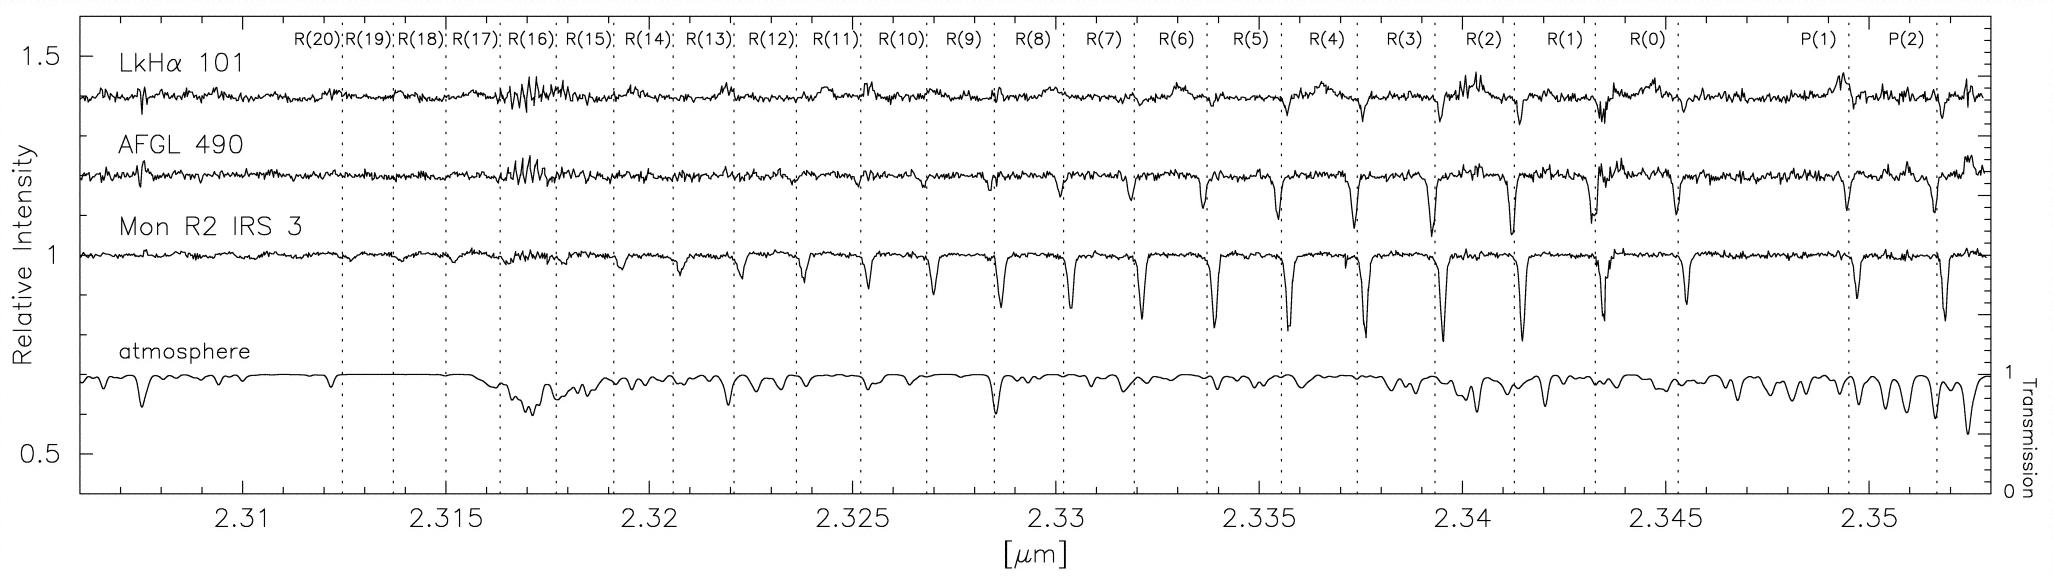
\includegraphics[width=\textwidth,height=!]{./B/CO_subaru_1.jpg}

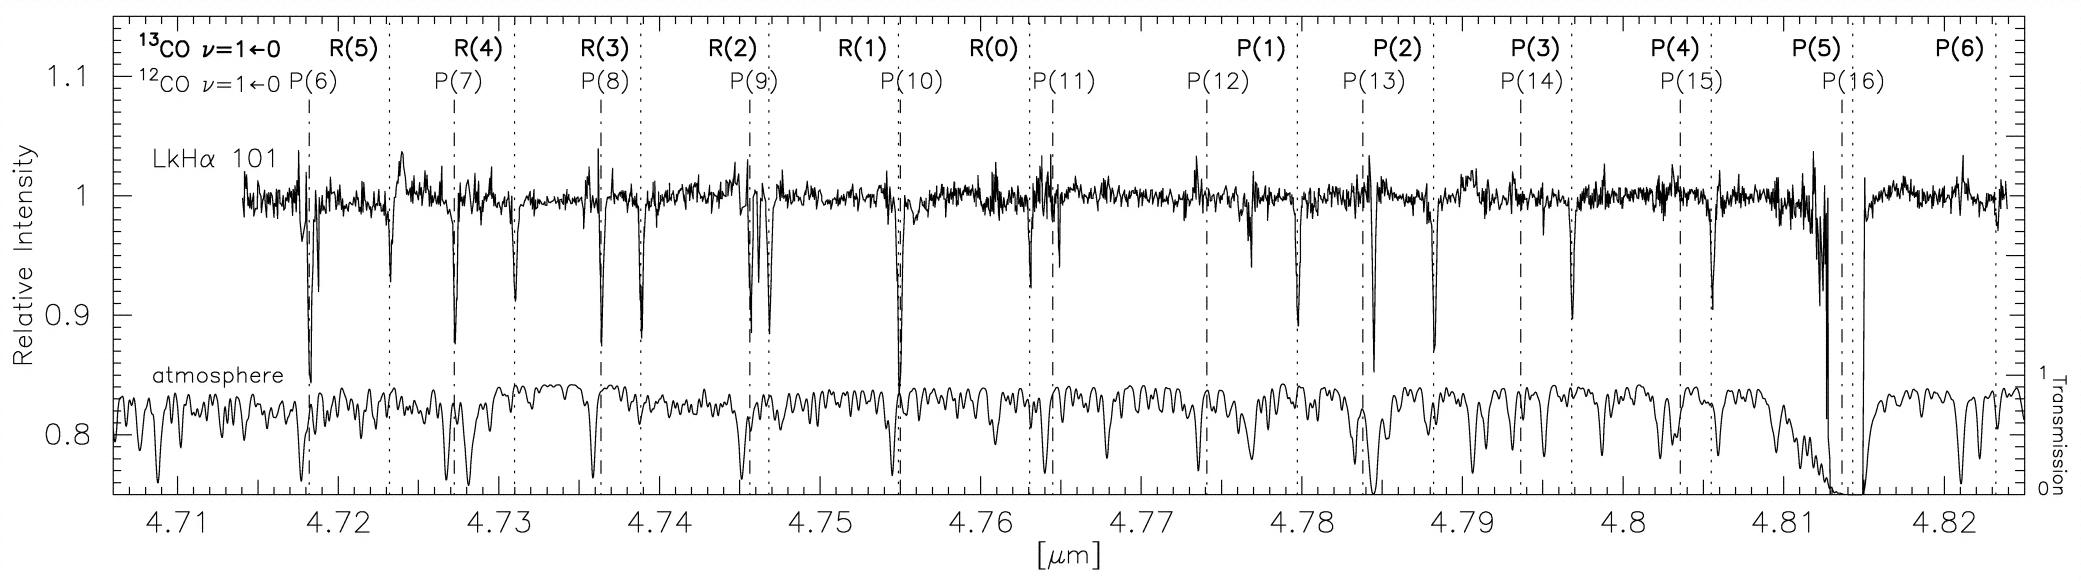
\includegraphics[width=\textwidth,height=!]{./B/CO_subaru_2.jpg}
\end{center}
\vfill



\end{frame} \begin{frame}\frametitle{Selection rules -- H$_2$}

In the case of $H_2$ we have $\vec{d}=0$. Moreover the fundamental
 state is $\vec{L} = 0$, and $\vec{S}=0$, so that $\vec{M}=0$ and all
 low-energy transitions for  $H_2$ are quadrupolar.

Note that the antisymmetry of the nuclear wave function implies that
the state $J=1$ ($J$ odd) is triplet ({\bf Ortho } H$_2$, $I =
S_\mathrm{nuclear} = 1$ ), while $J=0$ ($J$ even) is singlet ({\bf
Para } H$_2$, $I = 0$).\\


In H$_2$ the exclusion principle \footnote{the requirement that the
  wave function be antisymmetric} forbids $\Delta J = 1$, unless the
transition involves a change in spin state. The spin transitions can
only occur through the exchange of protons in collisions. Radiative
transitions between spin states can occur, but at a rate corresponding
to the quadrupolar transitions in the Hamiltonian of the deviations to
the Born-Oppenheimer approximations. \\


\end{frame} \begin{frame}\frametitle{}

In the ISM, {\bf Ortho } and {\bf Para } H$_2$ are effectively
different molecules. The distinction extends to all molecules that
contain H$_2$ radicals.

Rovibrational transitions between an upper level $^1$ and a lower
level $^2$ are written $(v_1-v_2)O(J_2)$, when $J_2-J_1 = -2$,
$(v_1-v_2)Q(J_2)$ when $J_2-J_1 = 0$, $(v_1-v_2)S(J_2)$ when $J_2-J_1
= +2$.



\end{frame} \begin{frame}\frametitle{H$_2$ energy levels}

\begin{minipage}[t]{0.59\textwidth}
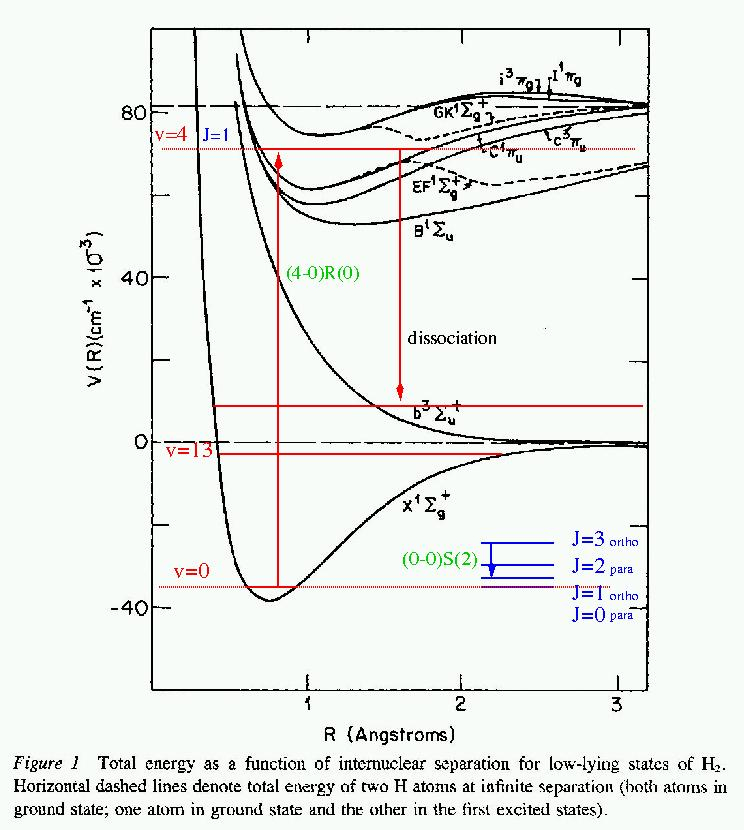
\includegraphics[width=\textwidth,height=!]{./B/h2_levels_xv.jpg}
\end{minipage}
\hfill
\begin{minipage}[t]{0.39\textwidth}
\vspace{-6cm}
$\Lambda = 0, 1, 2, ... $\\ $\Leftrightarrow$ $ \Sigma, \Pi, \Delta$ \\
levels in  $E_\mathrm{el}(R)$:\\ $X,B,C,D$.\\

The energy separation between levels $B$ and $C$ with respect to $X$
are $\sim$ 11~eV and 14~eV.  \\
\end{minipage}
\vfill

%
%\end{frame} \begin{frame}\frametitle{Emisi\'on IR de H$_2$}
%
%\begin{minipage}[t]{13cm}
%Como la tasa de transiciones radiativas en el nivel electr\'onico
%fundamental de H$_2$ es de orden cuadrupolar, la poblaciones de los
%niveles ro-vibracionales es dominada por colisiones entre moleculas de
%H$_2$. \\
%
%El n\'umero de ocupaci\'on de los niveles de energ\'{\i}a en el nivel
%fundamental de H$_2$ esta bien descrito por LTE:
%\[ N(v,J) \propto \omega(J) \exp(-B\,(J\,(J+1))/kT), \]
%en que $\omega(J) = 3 \times (2J+1) $ para ortho-$H_2$, y $\omega(J) =
%1 \times (2J+1) $ para para-$H_2$. 
%
%\end{minipage}
%\hfill
%\begin{minipage}[t]{10cm}
%\begin{center}
% \includegraphics[width=8cm,height=8cm]{./helix_ltepop.pdf}
%\end{center}
%\end{minipage}
%\vfill
%





\end{frame} 

\begin{frame}\frametitle{Dissociation of  H$_2$}

The collisional dissociation of  H$_2$,
\[\mathrm{H}_2 + \begin{array}{c}\mathrm{He}\\\mathrm{H}\\\mathrm{e}
\end{array} \rightarrow 2\mathrm{H} +  \begin{array}{c}\mathrm{He}\\\mathrm{H}\\\mathrm{e}
\end{array},\] requires temperatures of order the binding energy of  H$_2$, $4\mathrm{.}48~\mathrm{eV}/k = 52000~$K
\footnote{the  law of mass-action does not change this
result because the number of continuum states accessible to both
products and reactants is similar, in contrast with 
ionisation, which is described by the Saha equation}.

But an H$_2$ cloud is more likely to be photo-dissociated before it
reaches 50\,000~K. The dissociation continuum of H$_2$ (i.e. free
states of H+H) starts 14.7~eV above the fundamental level of H$_2$
(i.e. X$^{1}\Sigma$, para-H$_2$), while the ionization continuum (the
ejection of one electron) starts at 15.4~eV. Both continua, ionising
and dissociating, lie above 13.6~eV. In the context of a molecular
cloud surrounded by H\,{\sc i}, the H$_2$ dissociating radiation is
completely absorbed by the Lyman continuum of H\,{\sc i}.

\end{frame} \begin{frame}\frametitle{Dissociation of H$_2$}

The likeliest mechanism for H$_2$ dissociation is absorption to the
robrivational bands of excited electronic states (e.g. B o C), and
\begin{enumerate}
\item subsequent  de-excitation to dissociated levels of lower energy
 (e.g. b$^3\Sigma$), or \label{it:1mecah2}
\item  decay to the vibrational continuum of electronic state X (with
$v \ge 14$), or  \label{it:2mecah2}
\item decay to excited levels of the fundamental state and subsequent
absorption to the dissociating continuum (one order of magnitude
slower than mechanisms 1) and 2)  
%%%%%\ref{it:1mecah2} and \ref{it:2mecah2}
, Stecher\& Williams 1967, ApJ 149, L29)
\end{enumerate}
  
\end{frame} \begin{frame}\frametitle{IR emission from  H$_2$}

Since the rate of radiative transitions within the ground state
electronic level of H$_2$ is quadrupolar, the distribution of
ro-vibrational population is dominated by collisions between H$_2$
molecules. \\

If $kT \gg \Delta E_\mathrm{FIR}$, the typical energy difference between
rotational levels of ground state H$_2$, the occupation numbers of the
robrivational levels in the ground state electronic state follow LTE:
\[ N(v,J) \propto \omega(J) \exp(-B\,(J\,(J+1))/kT), \]
in which $\omega(J) = 3 \times (2J+1) $ for ortho-$H_2$, and $\omega(J)
= 1 \times (2J+1) $ for para-$H_2$. This situation (i.e. hot molecular
gas) is typical of shocks in the ISM.

In the presence of an intense UV field the IR emission of H$_2$ is
fluorescent (Black \& Van Dishoeck, 1987, ApJ, 322, 412). Fluorescence
dominates if $kT \ll \Delta E_\mathrm{FIR}$. The absorption of one UV
photon excites H$_2$ to an electronic state, leading to
photodissociation (with a 15\% probability), and to an IR cascade in
all other cases.





\end{frame} \begin{frame}\frametitle{IR emission from H$_2$}

Example excitation diagram for the Helix nebula.

\begin{center}
\includegraphics[width=0.8\textwidth,height=!]{./B/helix_ltepop.pdf}
\end{center}

\end{frame} 

\begin{frame}\frametitle{IR emission from H$_2$, $\zeta$~Oph}
\vspace{-1.5cm}
\begin{center}
\rotatebox{-90}{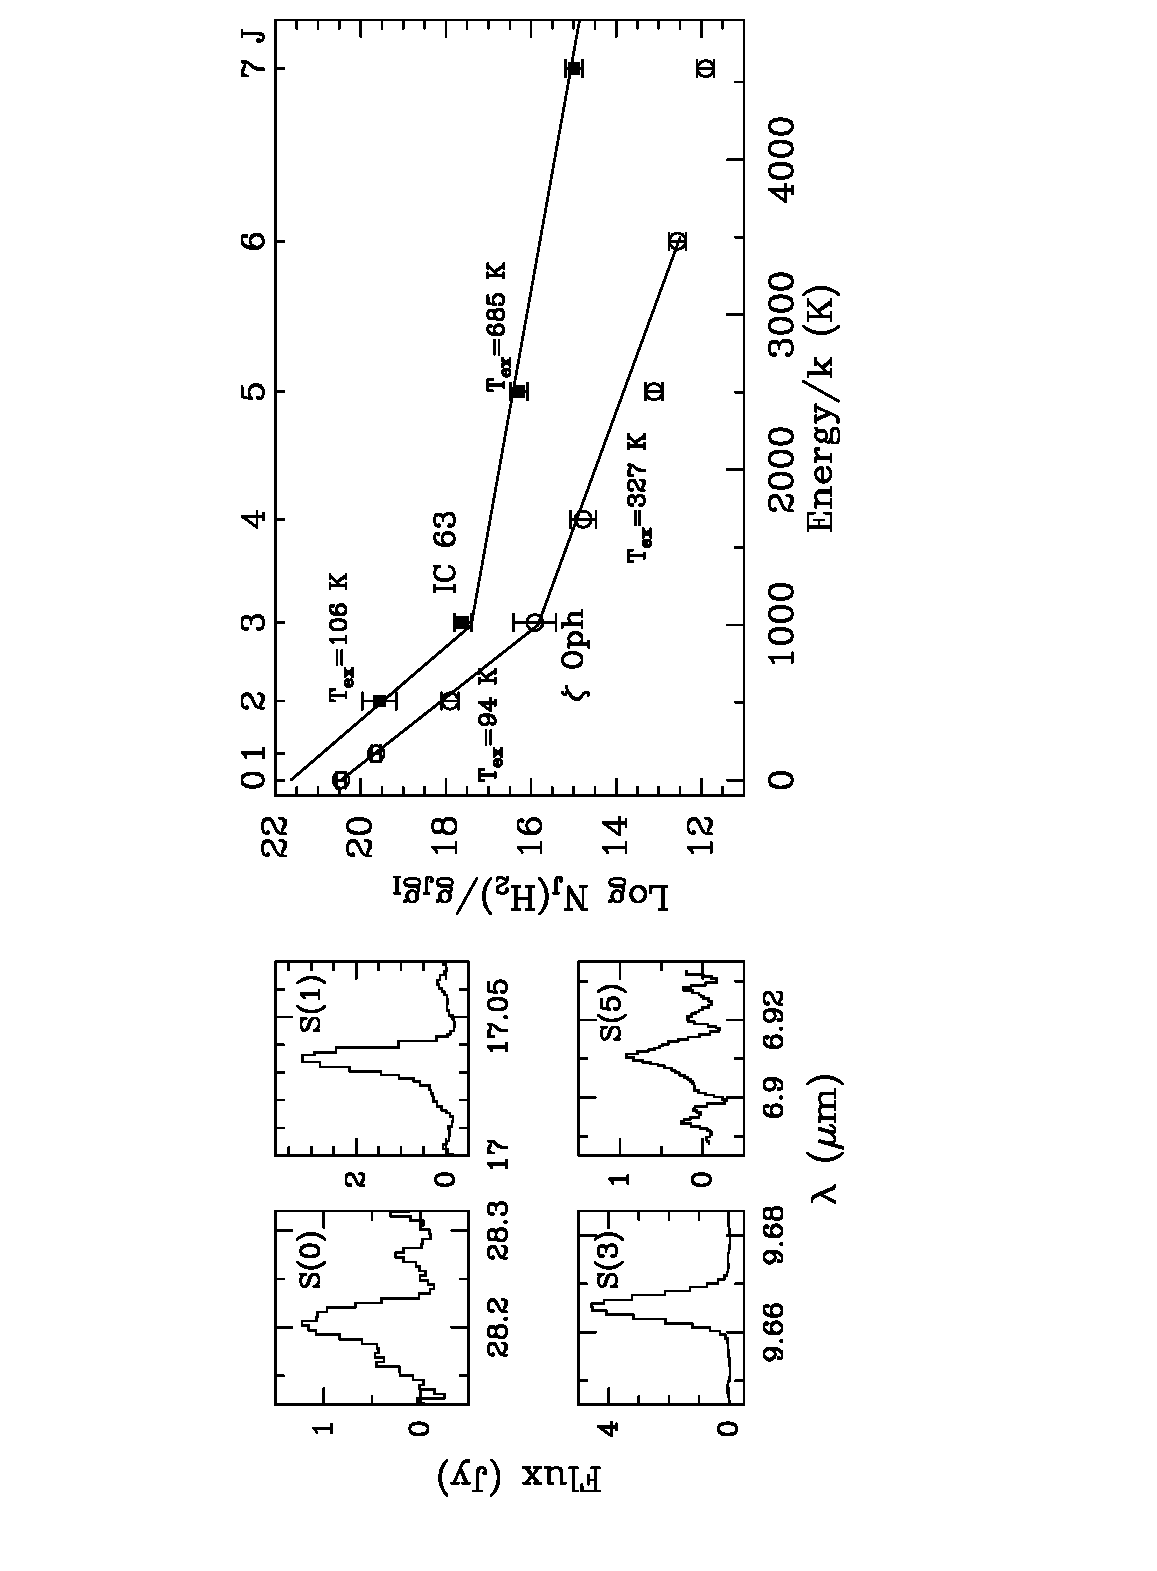
\includegraphics[width=0.7\textwidth,height=!]{./B/dishoeck_fig13.pdf}}

\vspace{-1.5cm}
\rotatebox{-90}{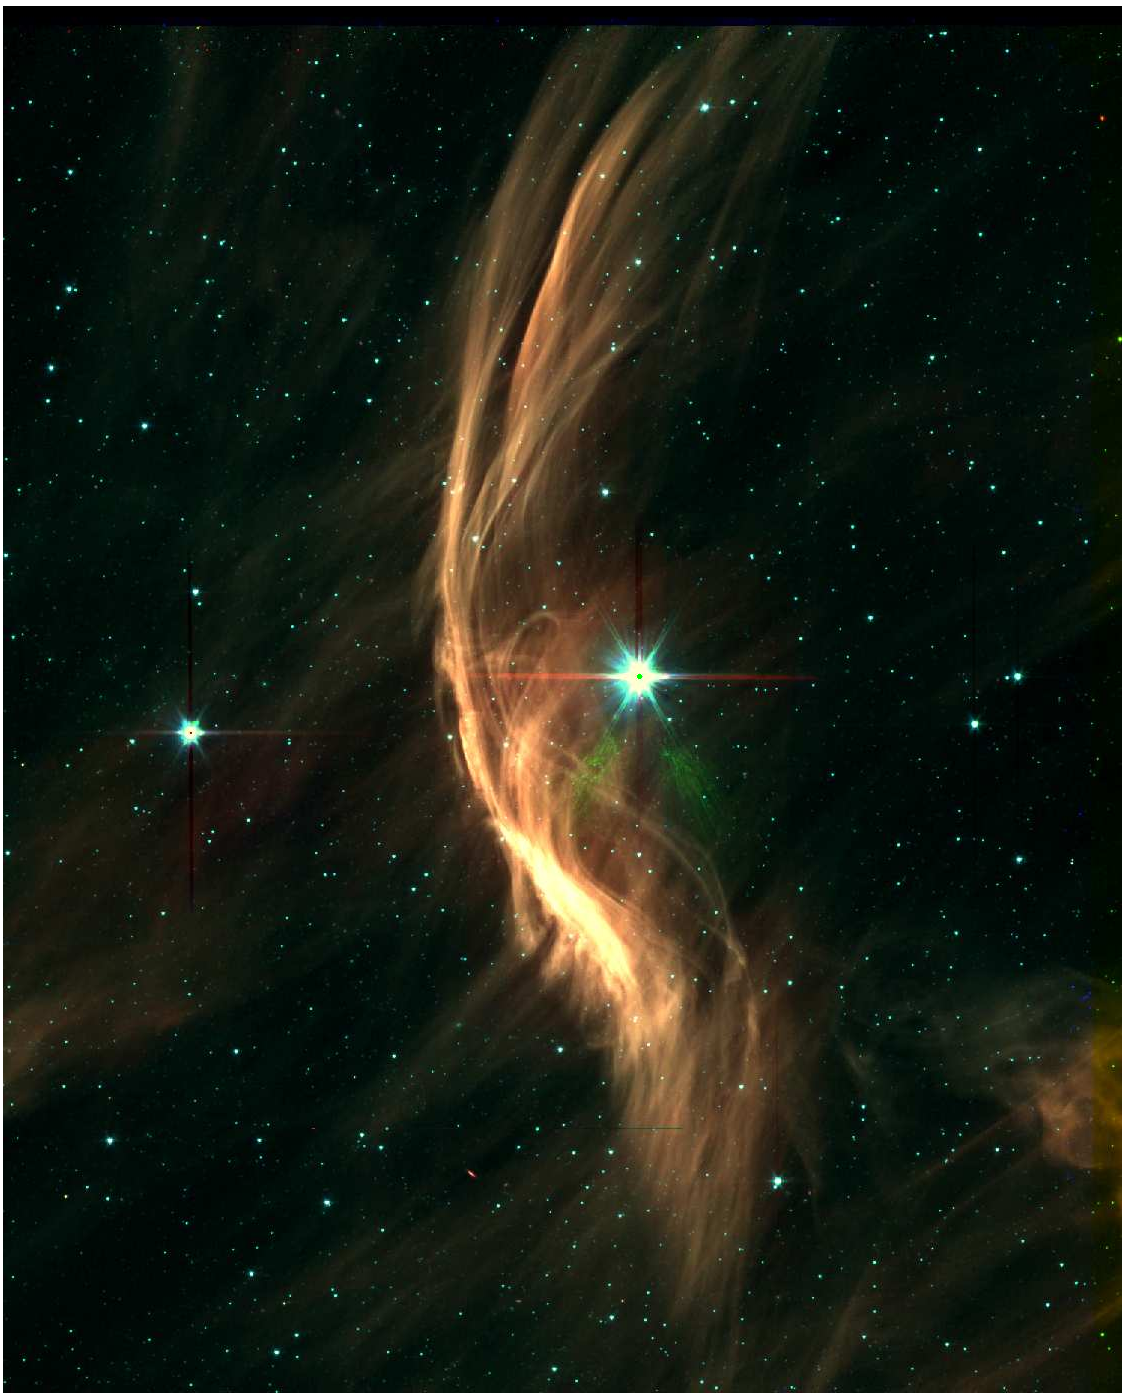
\includegraphics[width=0.4\textwidth,height=!]{./B/ZOPH_IRACrgb.pdf}}
\end{center}


%\begin{center}
%\end{center}
%
\vfill
              
%%%%%%%%%%%%%%%%%%%%%%%%%%%%%%%%%%%%%%%%%%%%%%%%%%%%%%%%%%%%%%%%%%%%%%%%%%%%%%%%%%
%%%%%%%%%%%%%%%%%%%%%%%%%%%%%%%%%%%%%%%%%%%%%%%%%%%%%%%%%%%%%%%%%%%%%%%%%%%%%%%%%%
%%%%%%%%%%%%%%%%%%%%%%%%%%%%%%%%%%%%%%%%%%%%%%%%%%%%%%%%%%%%%%%%%%%%%%%%%%%%%%%%%%

\end{frame}


\subsection{Heating of the ISM}

 \begin{frame}\frametitle{Heating of the neutral ISM}

H$_2$ is an important source of UV opacity, as shown in the {\em FUSE}
spectra of HD210839 and HD154368 (Rachford et al., 2002, ApJ, 577,
221).

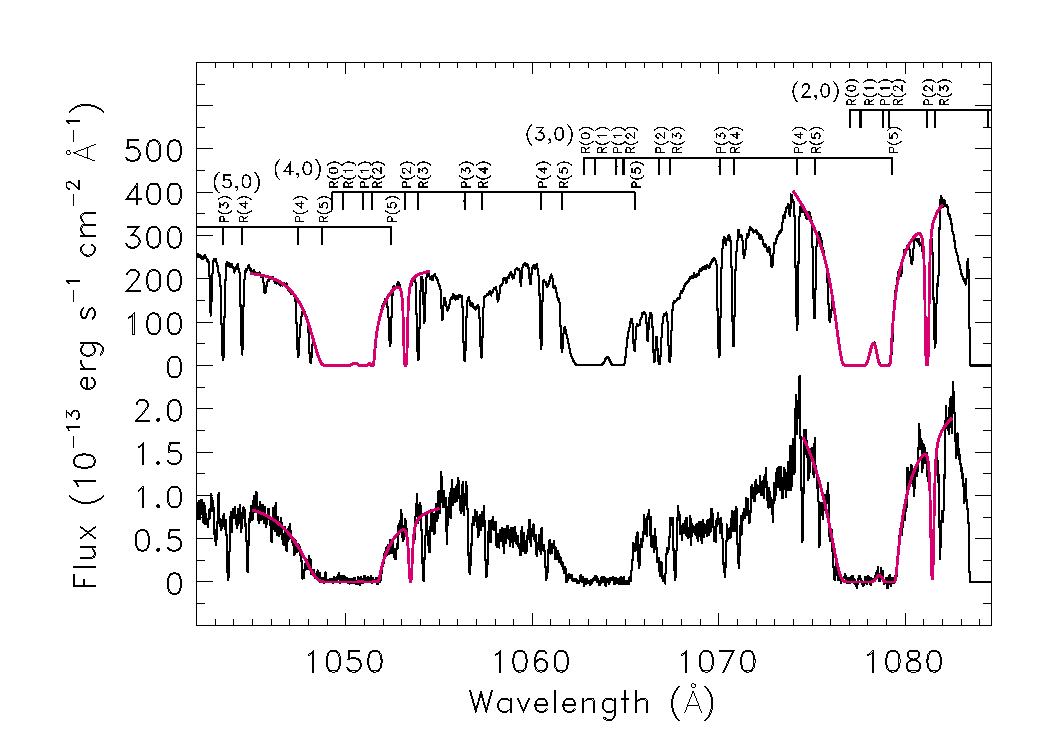
\includegraphics[width=\textwidth,height=!]{./B/fuse_H2}
\vfill

\end{frame} \begin{frame}\frametitle{Heating mechanisms}

\begin{enumerate}

\item Photoionisation: 
\[A ~  + ~h\nu ~\rightarrow~ A^+ + e, \]
in the case of the neutral ISM, photoionisation heating is dominated
by C$^+$, with an ionization potential of 11.3~eV. The average kinetic
enery of the ejected electron is 
\[ \frac{3}{2}kT_i = \frac{\int_{\nu_i}^{\infty} (J(\nu)/h\nu) \alpha_i(\nu) h(\nu
-\nu_i) d\nu}{\int_{\nu_i}^{\infty} (J(\nu)/h\nu) \alpha_i(\nu)d\nu
 }. \]

\item Photodissociation: 
\[AB ~  + ~h\nu ~\rightarrow~ A +~ B + KE, \]
dominated by $H_2$ photodissociation.
\item collisional de-excitation (in particular for H$_2$, when  
$n(\mathrm{H}_2) > 10^4~$cm$^{-3}$).
\seti
\end{enumerate}

\end{frame} \begin{frame}\frametitle{}

\begin{enumerate}
\conti
\item photoelectric effect on dust grains. \\
The grain heating efficiency, $\epsilon_\mathrm{grain}$, defined as the
ratio between output gas heating and input UV radiation (Tielens
Chap. 3.3.1), is 
\[ \epsilon_\mathrm{grain} =  Y \times \frac{h\nu - W - \phi }{h\nu}
,\]

where the electron escape probability $Y$ is the ratio between the
e$^-$ - e$^-$ mean free path $l_e \approx 10~$\angstrom, and the
absorption depth of UV radiation, $l_a \approx 100~$\angstrom :
$Y \approx l_e /l_a$.  $W$ is the work function of the grain and $\phi
= Z \times e^2 / a$ is the surface potential for a grain of size
$a$. The ionization potential of a grain is thus $ I = W + \phi$. \\
The heating efficiency is larger for smaller grains, since
$l_a \approx l_e$.  {\large The ejection of photoelectrons from grains
is the dominant heating source in the neutral ISM exposed to FUV
radiation, as in the case of PDRs. Photoionisation is dominant in the
case of the ionised gas.}
\seti
\end{enumerate}


\end{frame} \begin{frame}\frametitle{}

\begin{itemize}
\item The total photoelectric  heating  rate from grains per unit volume, $n\,\Gamma_\mathrm{grain}$, can be written:
\[ n\,\Gamma_\mathrm{grain} = \int_{a_\mathrm{min}}^{a_\mathrm{max}}
n(a) da \sum_i \int_{\nu_i}^{\nu_\mathrm{H}} \frac{J_\nu}{h\nu}
\alpha_\mathrm{grain,i}(\nu) E_\mathrm{kin}(a,i) d\nu   , \]
where $a$ is grain diameter, and $i$ runs over grain ionisation stage,
and $ h \nu_\mathrm{H} = 13.6~$eV.

\item in addition to photo-electric heating, grains can also heat the
gas through inelastic collisions if the solid state temperature is
larger than the gas temperature. 
\end{itemize}
 

\end{frame} \begin{frame}\frametitle{}


\begin{enumerate}
\conti
\item heating from cosmic rays:\\
Important for molecular phase. Cosmic rays, as well as X-rays, ionise H$_2$ (IP=15.4~eV):
\[ \mathrm{H}_2 + (p,e^-,\alpha,X) \rightarrow \mathrm{H}_2^+ + e^- +  (p,e^-,\alpha,X)^\prime,
\]
followed by the formation of $\mathrm{H}_3^+$:
\[ \mathrm{H}_2^+ +   \mathrm{H}_2 \rightarrow \mathrm{H}_3^+ + \mathrm{H}. \]
An important mechanism for the destruction of H$_3^+$ is its
dissociative recombination,
\[ \mathrm{H}_3^+ + e \rightarrow \left\{ \begin{array}{c} 3\mathrm{H} \\
  \mathrm{H}_2 + \mathrm{H} \end{array} \right. \] Since both the
  formation and the destructionof H$_3^+$ are exothermic (the energy
  released into the ISM in the process is 11~eV), the 
  H$_3^+$ cycle is a heating source of the ISM.
\seti
\end{enumerate}

\end{frame} \begin{frame}\frametitle{}


\begin{enumerate}
\conti
\item Turbulent heating.

Important in molecular clouds at $\sim 10~$K, without UV field. 


In a turbulent flow the kinetic energy density will trickle down a
hierarchy of scales, until it is dissipated by diffusion at the
smallest scale fixed by viscosity. The timescale for downwards energy
transfer at scale $l$ can be approximated with the crossing time at
the velocity disperson $v$. Thus the rate of heating per unit volume
is (Tielens 3.8),
\[ n \Gamma_\mathrm{turbulence} = \frac{1}{2} \frac{n ~ m_\mathrm{H}
v^2}{l/v} . \]

The observations of the energy density and velocity dispersion at a
given scale $l$ leads to an estimate of turbulent heating. 

The energy densities as a function of scale can be calculated assuming
a constant energy transfer rate: $ v^2 / (l/v)$ is constant. 
\seti
\end{enumerate}

\end{frame} \begin{frame}\frametitle{Heating mechanisms in neutral diffuse clouds}

\rotatebox{0}{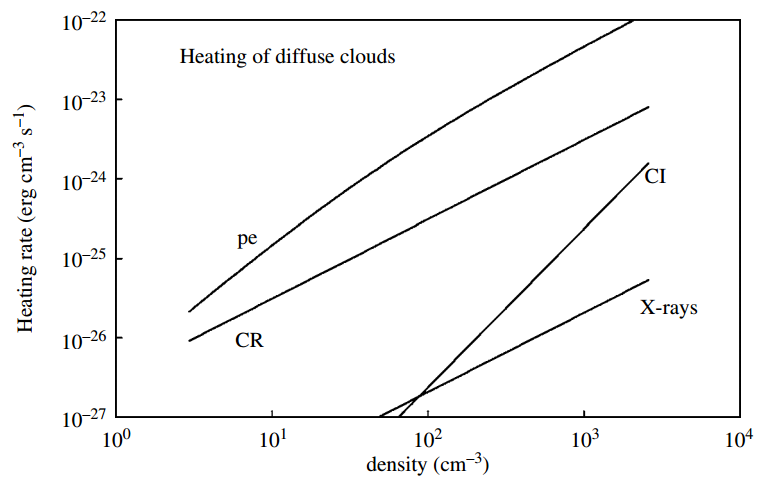
\includegraphics[width=0.9\textwidth,height=!]{./B/heating_DC.png}}

\end{frame} \begin{frame}\frametitle{Heating mechanisms in WNM}

\rotatebox{0}{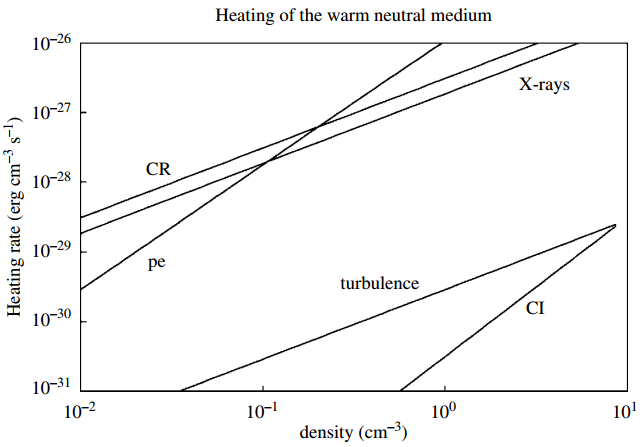
\includegraphics[width=0.9\textwidth,height=!]{./B/heating_WNM.png}}

\end{frame} \begin{frame}\frametitle{Heating mechanisms in molevular clouds}

\rotatebox{0}{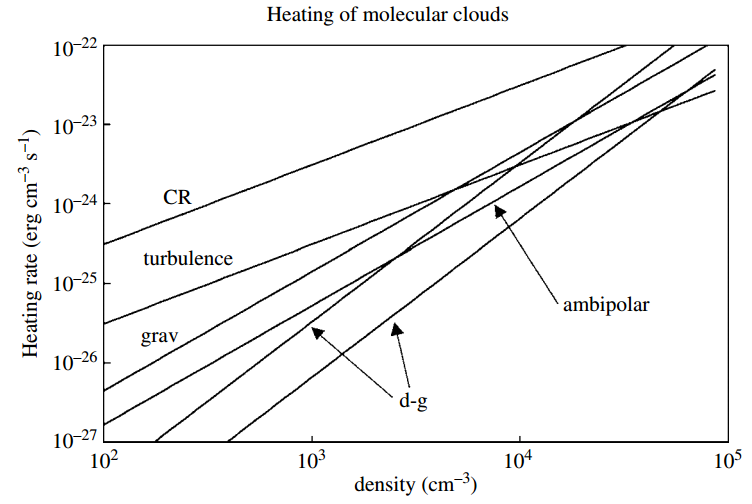
\includegraphics[width=0.9\textwidth,height=!]{./B/heating_MC.png}}

\end{frame} \begin{frame}\frametitle{Steady state temp. for HI}

\rotatebox{0}{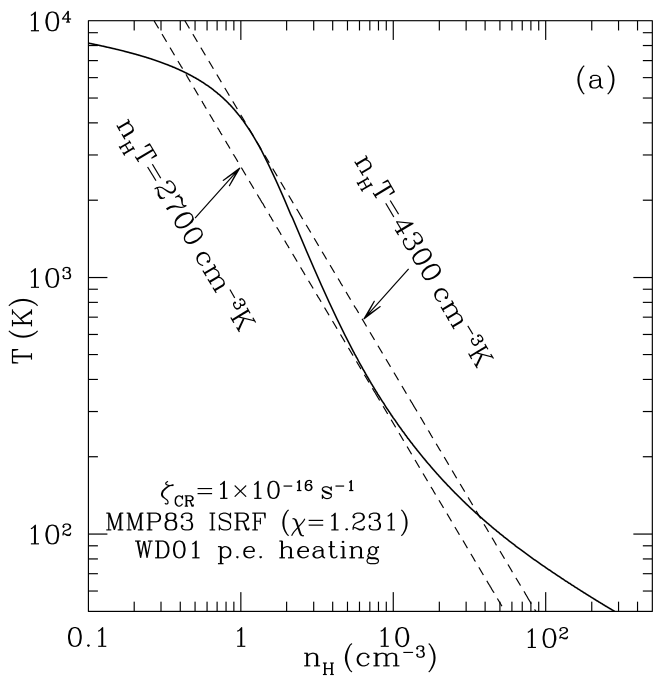
\includegraphics[width=0.8\textwidth,height=!]{./B/temp_nh.png}}

\end{frame} \begin{frame}\frametitle{Two phases for HI}

\rotatebox{0}{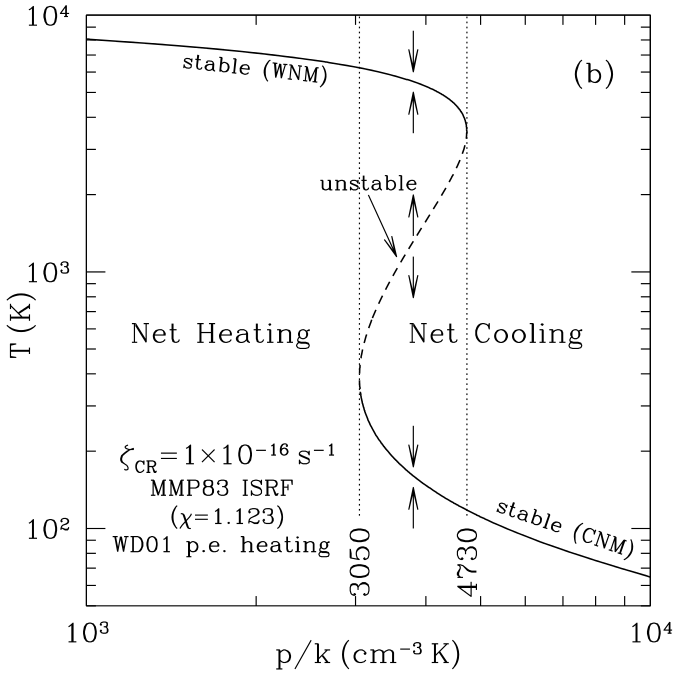
\includegraphics[width=0.8\textwidth,height=!]{./B/temp_p.png}}

\end{frame}

\section{Molecule formation}

\subsection{Grain catalysis}

\begin{frame}\frametitle{Molecule formation}



The encounter of two atoms $A$ and $B$, initially unbound, will lead
to molecular synthesis if:
\begin{enumerate}
\item bound states of $AB$ exist.

\item There is a mechanism for molecular stabilization faster than the
lifetime of the $AB^\star$ state \footnote{the molecule is initially
bound at a level with energy equal to that of the colliding pair}, of
order  $\sim 10^{-13}$~s ($\approx 1$ vibrational period).
\end{enumerate}


Radiative dissipation of the energy excess of $AB^\star$ is
improbable: even for electric dipole decay rates, about
$10^8~$s$^{-1}$ in the UV, only 1 out of $10^5$ collisions will produce
a molecule.\\  

The abundance of H$_2$ might raise the low probability of condensation
via collisions, but the electric dipole transitions of H$_2$ are
fobbiden. H$_2$ cannot associate radiatively.\\

The H$_2$ half-life in the diffuse interstellar UV radiation field is
of $\sim 300~$yr $\Rightarrow$ some other mechanism must exist for
efficient H$_2$ formation. 


\end{frame} \begin{frame}\frametitle{Grain catalysis of the formation process of  H$_2$}

The adsorption of hydrogen atoms onto the surface of dust grains
allows raising the available timescale for the $A$~+~$B$ encounter,
and the grain acts as stabilizing agent by absorbing the excess energy
of $AB^\star$. 

Once H$_2$ is formed, its 4.48~eV of binding energy (the first
bound-free transition is at 2500~\angstrom) eject H$_2$ from the grain
surface, and the excess of energy over the grain work function is
distributed over the molecular degrees of freedom, leaving the H$_2$
molecule in an excited state. 


IR transitions from the formation pumping of excited levels of H$_2$
were observed by Burton et al. (2002, MNRAS, 333, 721) in M~17: the
line (6-4)O(3) at 1.73$\mu$m cannot be collisionally excited since its
superior level is at $\Delta E/k$$\sim$30\,000~K above ground, yet the
intensity of (6-4)O(3) relative to other H$_2$ lines does not match
fluorescent models.

\end{frame} 

\subsection{Ion-molecule chemistry}

\begin{frame}\frametitle{Molecule formation - the
role of H$_3^+$}

$\bullet$ H$_3^+$ controls the ionisation stage of the molecular ISM. \\

The  H$_3^+$  cycle with corresponding rates is:
\[ \mathrm{H}_2 + (p,e^-,\alpha,X) \stackrel{\zeta}{\rightarrow}
\mathrm{H}_2^+ + e^- +  (p,e^-,\alpha,X)^\prime, \]
\[ \mathrm{H}_2^+ +   \mathrm{H}_2 \stackrel{\eta_1} {\rightarrow} \mathrm{H}_3^+ + \mathrm{H}, \]
\[ \mathrm{H}_3^+ + e \stackrel{\eta_2}{\rightarrow}    \mathrm{H}_2 +
\mathrm{H}, \]
where $\zeta$ is the ionization rate of H$_2$, in s$^{-1}$. We see that  
\[ \zeta n_{\mathrm{H}_2} = \eta_1 n_{\mathrm{H}_2}
n_{\mathrm{H}^+_2}, \text{~and} \] 
\[ \eta_2 n_{\mathrm{H}_3^+} n_e =  \zeta n_{\mathrm{H}_2}   \] 
With canonical values for the rates $\eta_i$, one gets
$n_{\mathrm{H}_3^+} \gg n_{\mathrm{H}_2^+}$, and the requisite for
neutrality $n_\mathrm{e} \approx n_{\mathrm{H}_3^+}$ allows concluding
$n_\mathrm{e} / n_{\mathrm{H}_2} \approx 10^{-8}~$.


\end{frame} \begin{frame}\frametitle{Ion-molecule chemistry}


$\bullet$ In ion-molecule chemistry, the standard model for
interstellar chemistry, H$_3^+$ is cornerstone to all reaction cycles:
\\ 

The cycle of an element X (anything short of He, O$_2$,...)  is 
initiated  by H$_3^+$ through 
\[ \mathrm{H}_3^+ + \mathrm{X} \rightarrow \mathrm{XH^+} + \mathrm{H}_2,~
\text{and subsequently,}\]
\[ \mathrm{XH^+} + \mathrm{Y} \rightarrow \mathrm{XY}^+ + \mathrm{H}
.\]

Example: production of $\mathrm{H_2O}$ and OH, \\
\[ \mathrm{H}_3^+ + \mathrm{O} \rightarrow \mathrm{OH^+} + \mathrm{H}_2,~
\text{followed by the sequence,}\]
\[ \mathrm{OH^+} + \mathrm{H}_2 \rightarrow \mathrm{OH_2}^+ +
\mathrm{H},  \]
\[ \mathrm{OH_2^+} + \mathrm{H}_2 \rightarrow \mathrm{OH_3}^+ +
\mathrm{H}, \]
 and finally one dissociative recombination  
\[ \mathrm{OH_3}^+ + \mathrm{e} \rightarrow \left\{ \begin{array}{l}
  \mathrm{H_2O} + \mathrm{H}\\ \mathrm{OH} + \mathrm{H_2} \end{array} \right. . \]




\end{frame} \begin{frame}\frametitle{The full story} 

$\bullet$  Molecular formation: realistic cycles (Sternberg \& Dalgarno 1995, ApJSS, 99, 565).


\begin{center}
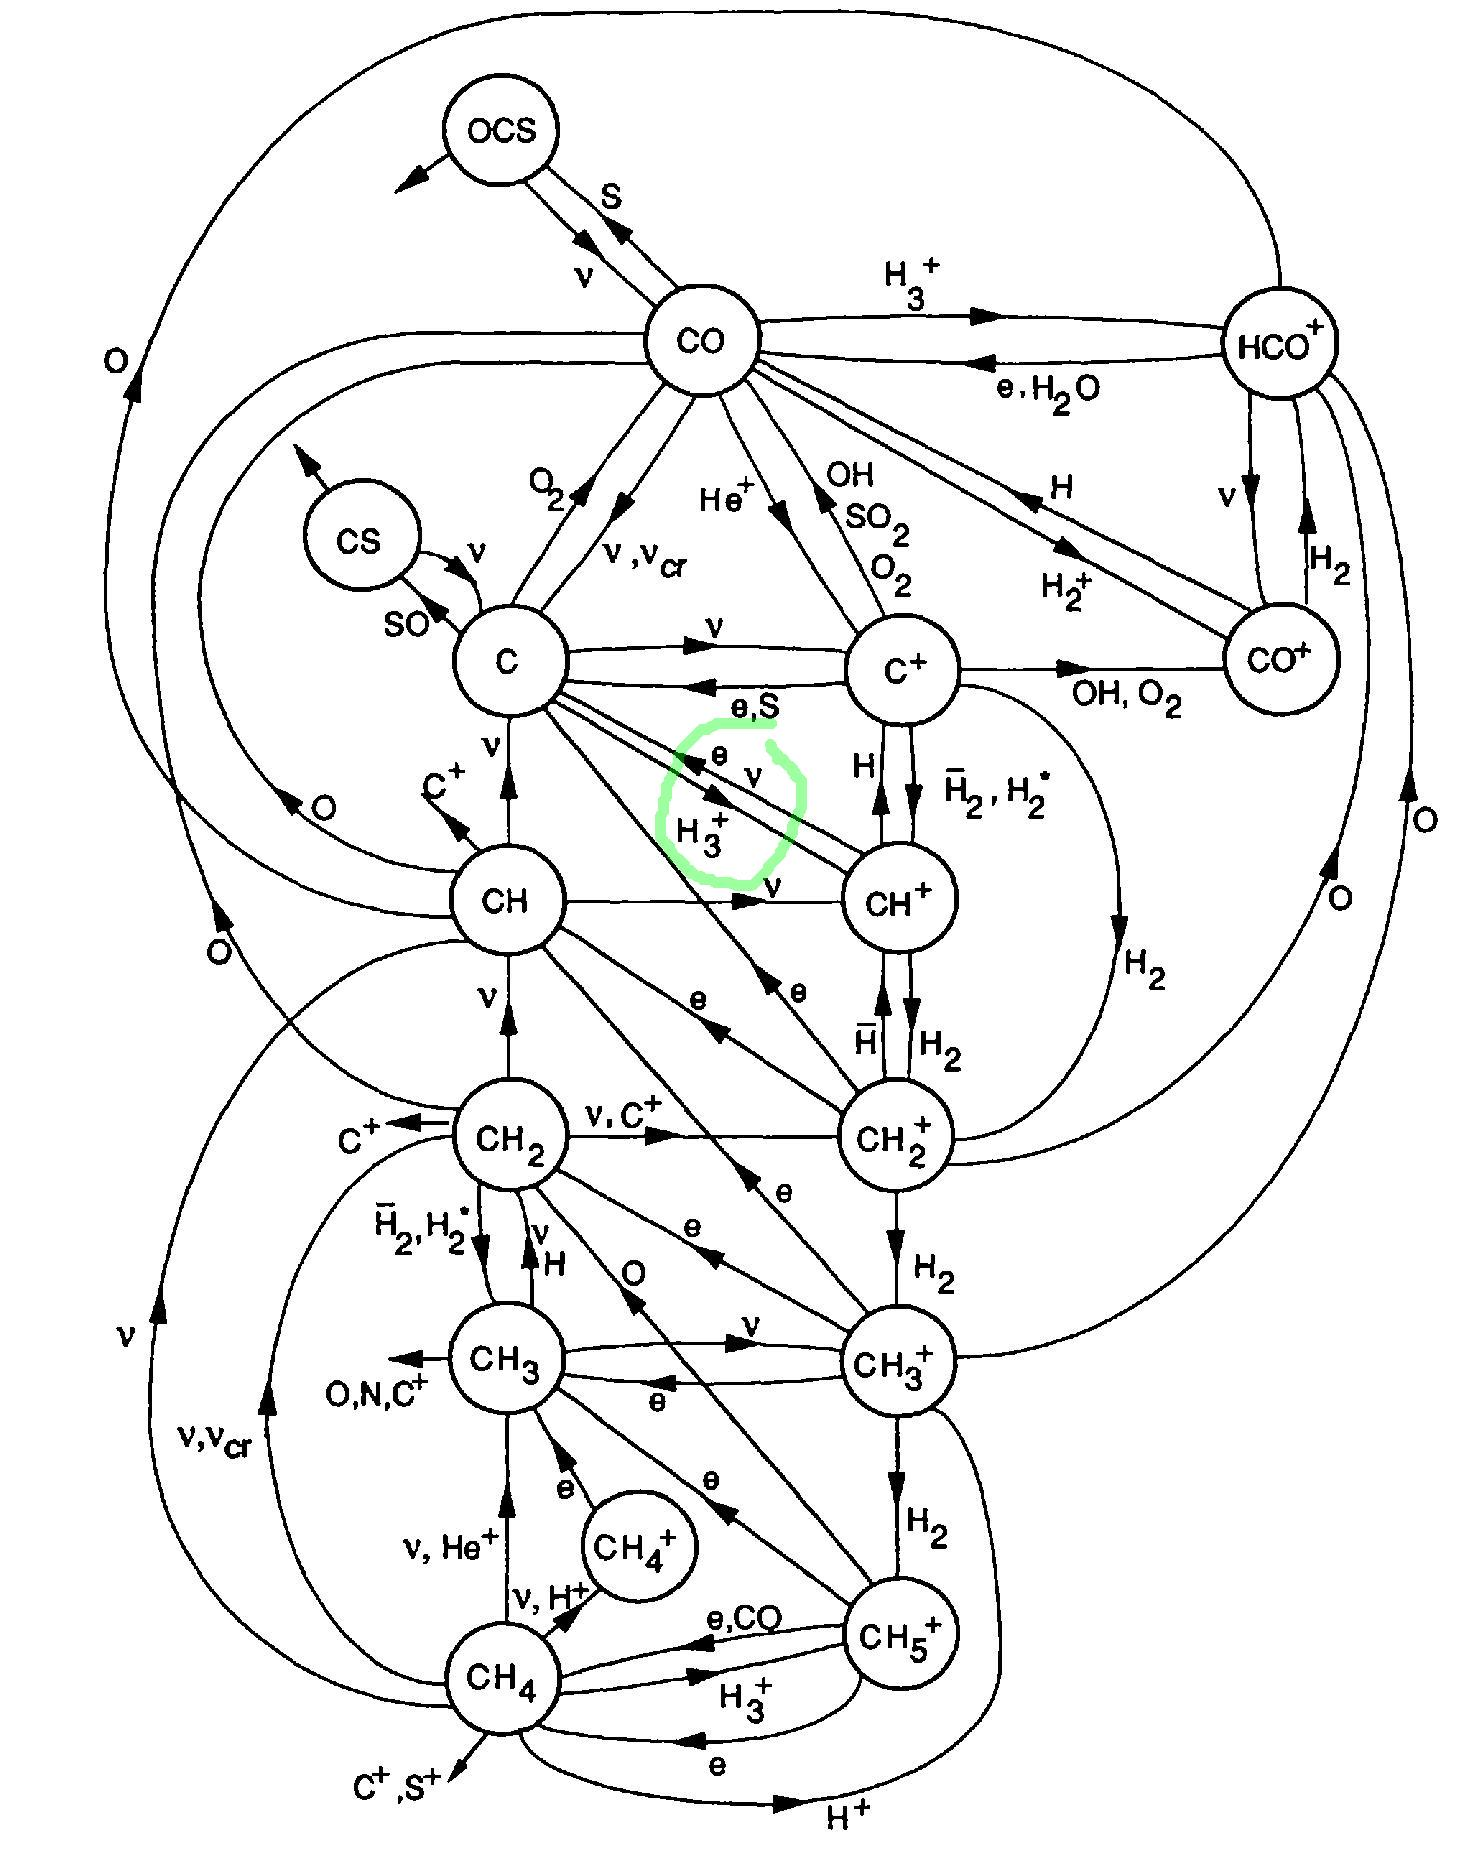
\includegraphics[width=0.6\textwidth,height=!]{./B/C_network_2.jpg}
\end{center}

\end{frame}

\subsection{Observational validation}

 \begin{frame}\frametitle{Molecular formation - validation of
the ion-molecule chemical model}

\begin{minipage}[t]{0.48\textwidth}
H$_3^+$, the pilar of chemical cycles in the ISM, was detected by
Geballe \& Oka (1996, {\em Nature}, 384, 334; Geballe 2000, {\em
Phil.Trans.R.Soc.Lond.}A, 358, 2503), with an abundance close to that
expected from the ionization fraction.

H$_3^+$ does not have electric dipole moments, and is even worse than
H$_2$: it is deprived of excited electronic states (i.e. no UV
transitions). It only has two vibration modes. One is symmetrical,
$\nu_1$, that does not induce electric dipole moment and does not
radiate. Only the asymmetrical mode $\nu_2$ induces an electric dipole.

\end{minipage}
\hfill
\begin{minipage}[t]{0.5\textwidth}
  \vspace{-0cm}
  \begin{center}
    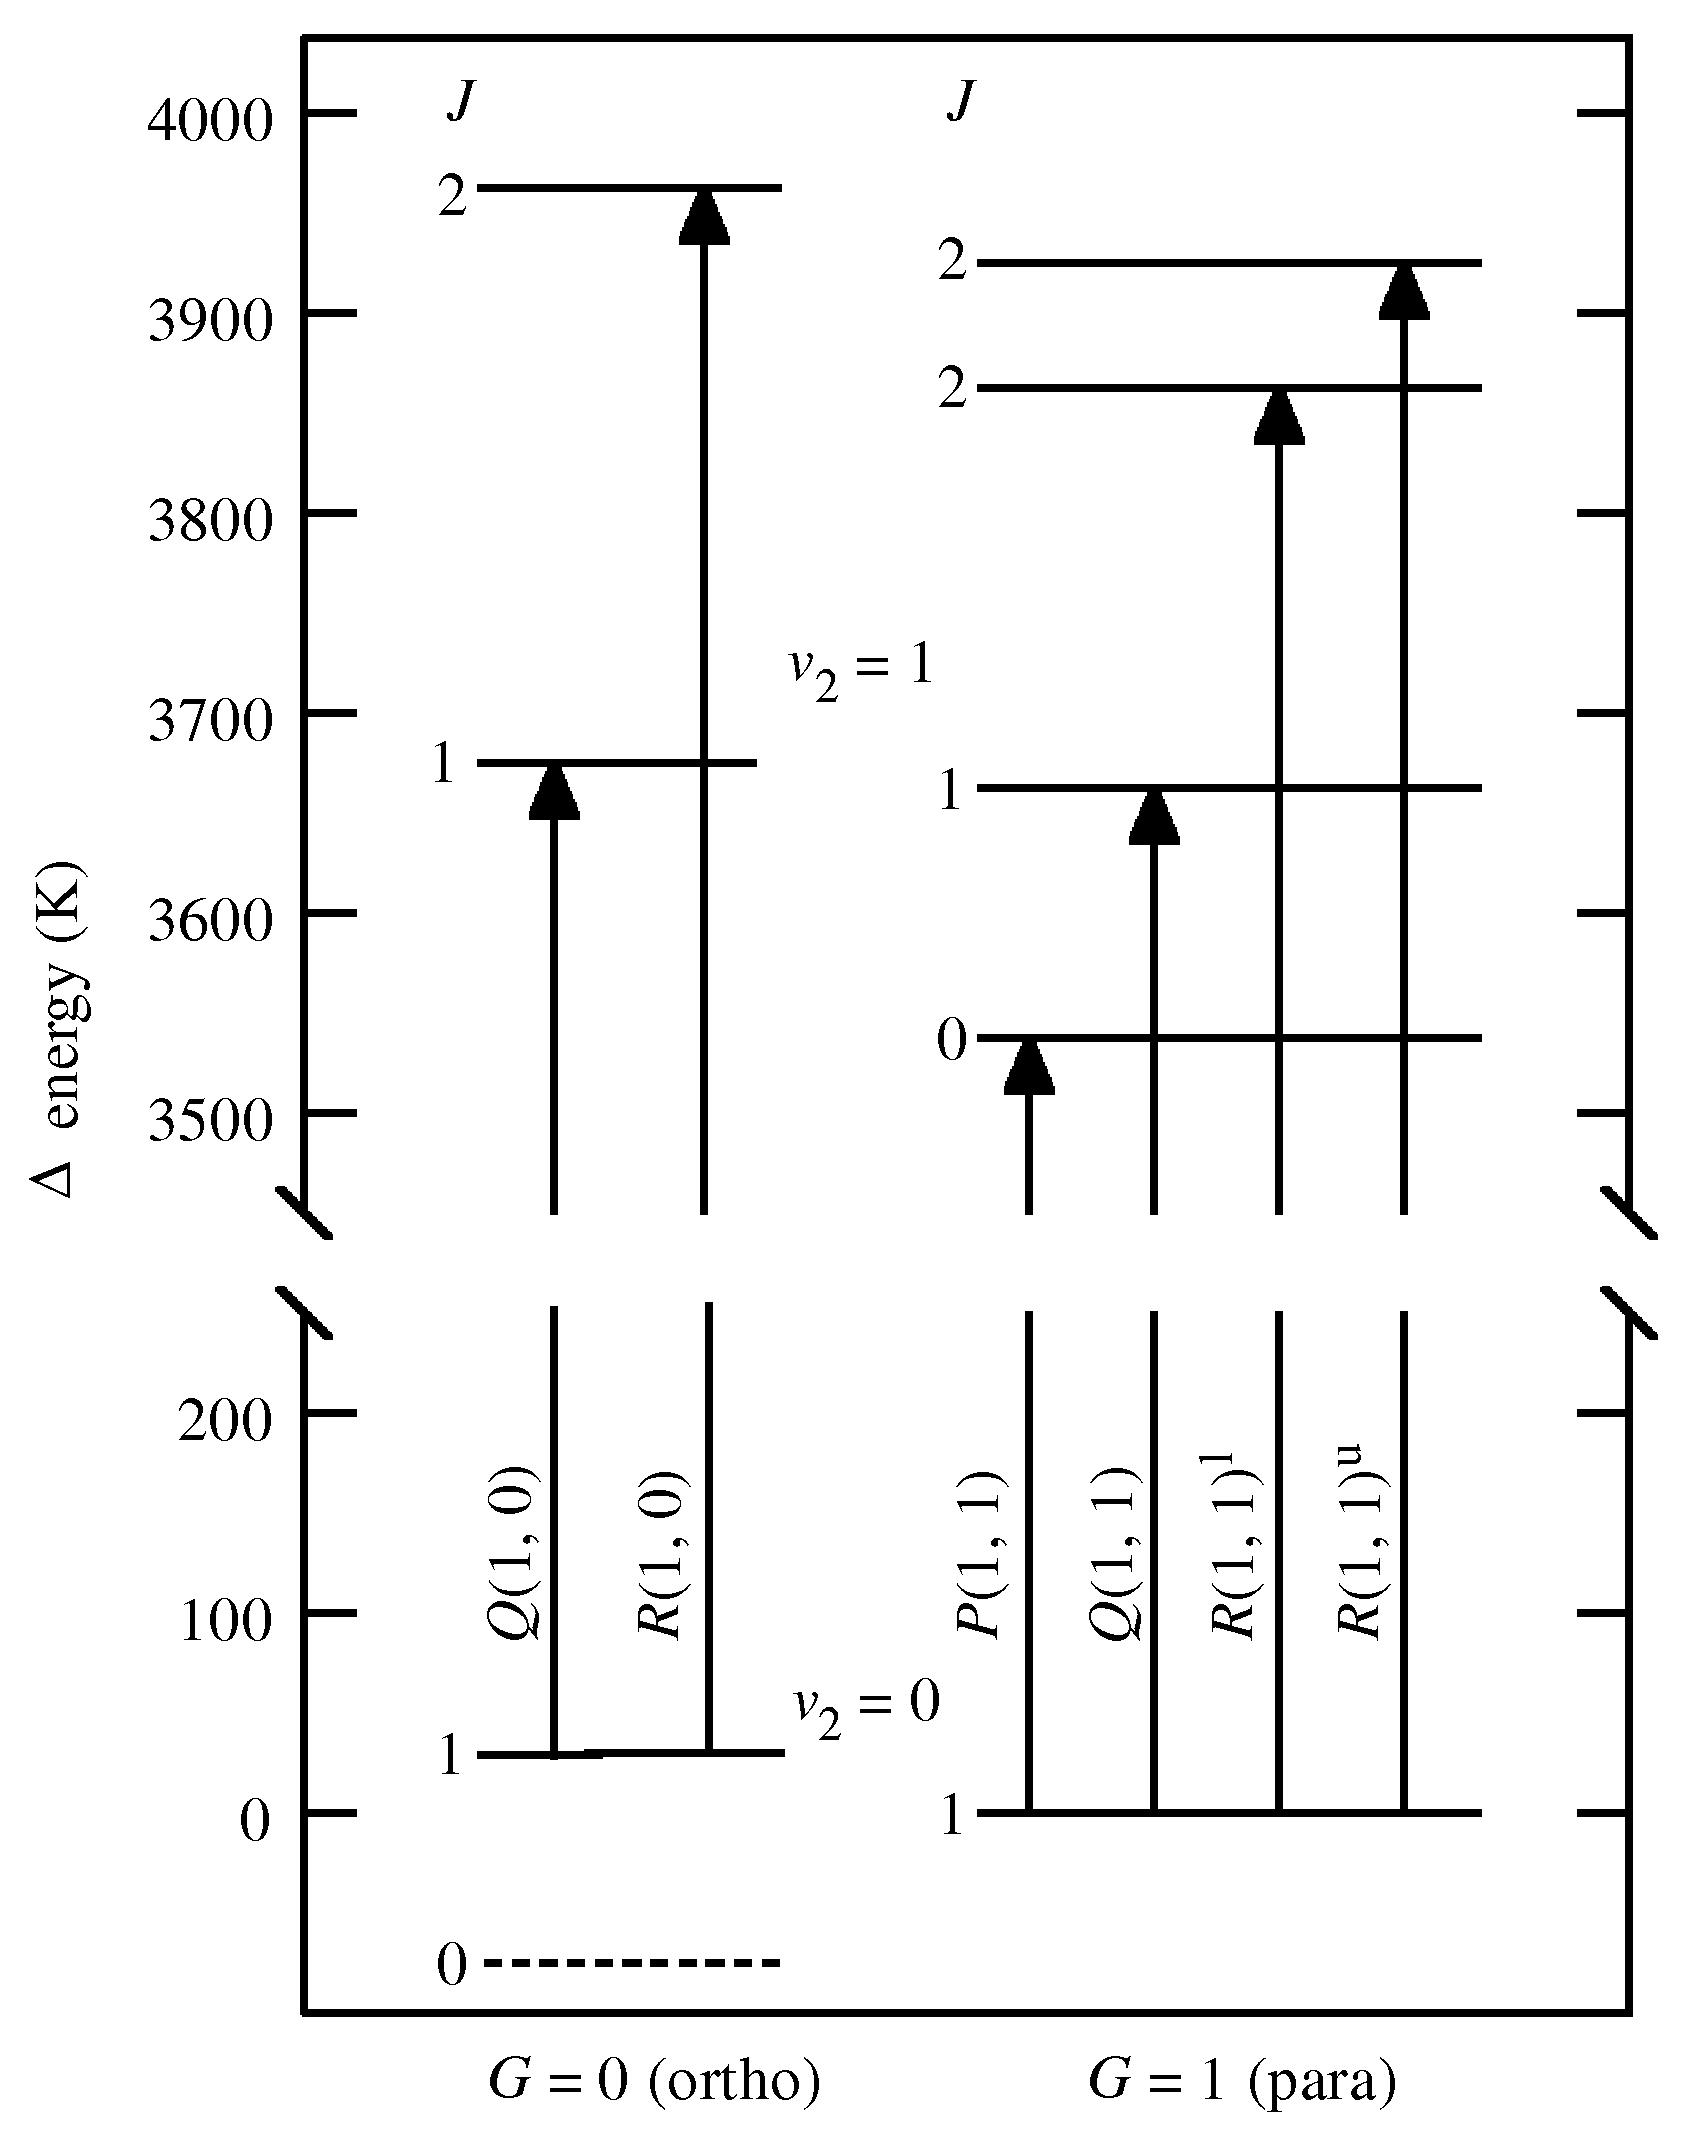
\includegraphics[width=\textwidth,height=!]{./B/h3_levels.jpg}
  \end{center}
\end{minipage}


%\textcolor{red}{B$_3$} Formaci\'on de mol\'eculas -
%  abundancia esperada de H$_3^+$  
\end{frame} 



\begin{frame}\frametitle{The production of  H$_3^+$}

 
\[ \mathrm{H}_2 + (p,e^-,\alpha,X) \stackrel{\zeta}{\rightarrow}
\mathrm{H}_2^+ + e^- +  (p,e^-,\alpha,X)^\prime, \]
\[\mathrm{H}_2^+ +   \mathrm{H}_2 \stackrel{\eta_2} {\rightarrow} \mathrm{H}_3^+ + \mathrm{H},\]
is balanced by its destruction, mainly through
\[ \mathrm{H}_3^+ + \mathrm{CO} \stackrel{\eta_\mathrm{CO}}{ \rightarrow} \mathrm{COH^+} +
\mathrm{H}_2, \]
equating rates, one gets
\[  \zeta n_\mathrm{H_2} = \eta_\mathrm{CO} n_\mathrm{H_3^+}
n_\mathrm{CO} ,\] in which $\eta_\mathrm{CO} = 1.8~10^{-9}~$s$^{-1}$,
and $\zeta = n_\mathrm{p,X,\alpha,e^{-}} ~\eta_1 \approx
3~10^{-17}~$s$^{-1},$ gives the product of the cosmic ray density
times the ionisation rate of H$_2$. In general the relative abundances
of CO and H$_2$ are constant in the diffuse ISM (model: Lee et al.,
1996, A\&AS, 119, 111, observations: Federman et al. 1980, ApJ 242,
545), $n_\mathrm{CO}/n_\mathrm{H_2} = 1.5~10^{-4}$, so that
\[ \boxed{ n_\mathrm{H_3^+}  \approx 10^{-4}~\mathrm{cm^{-3}}, ~~\text{independent of $n_\mathrm{H_2}$}} \]
For typical densities  $n_\mathrm{H_2} \approx 10^{4}
\mathrm{cm^{-3}}$, we have $N_{\mathrm{H}_3^+} \approx 10^{-9} N_{\mathrm{H}_2}~~~ \text{!!}$




%\textcolor{red}{B$_3$} Formaci\'on de mol\'eculas -
%  detecci\'on de H$_3^+$ 

\end{frame} \begin{frame}\frametitle{Detection of H$_3^+$, Oka \& Geballe }
\begin{center}
  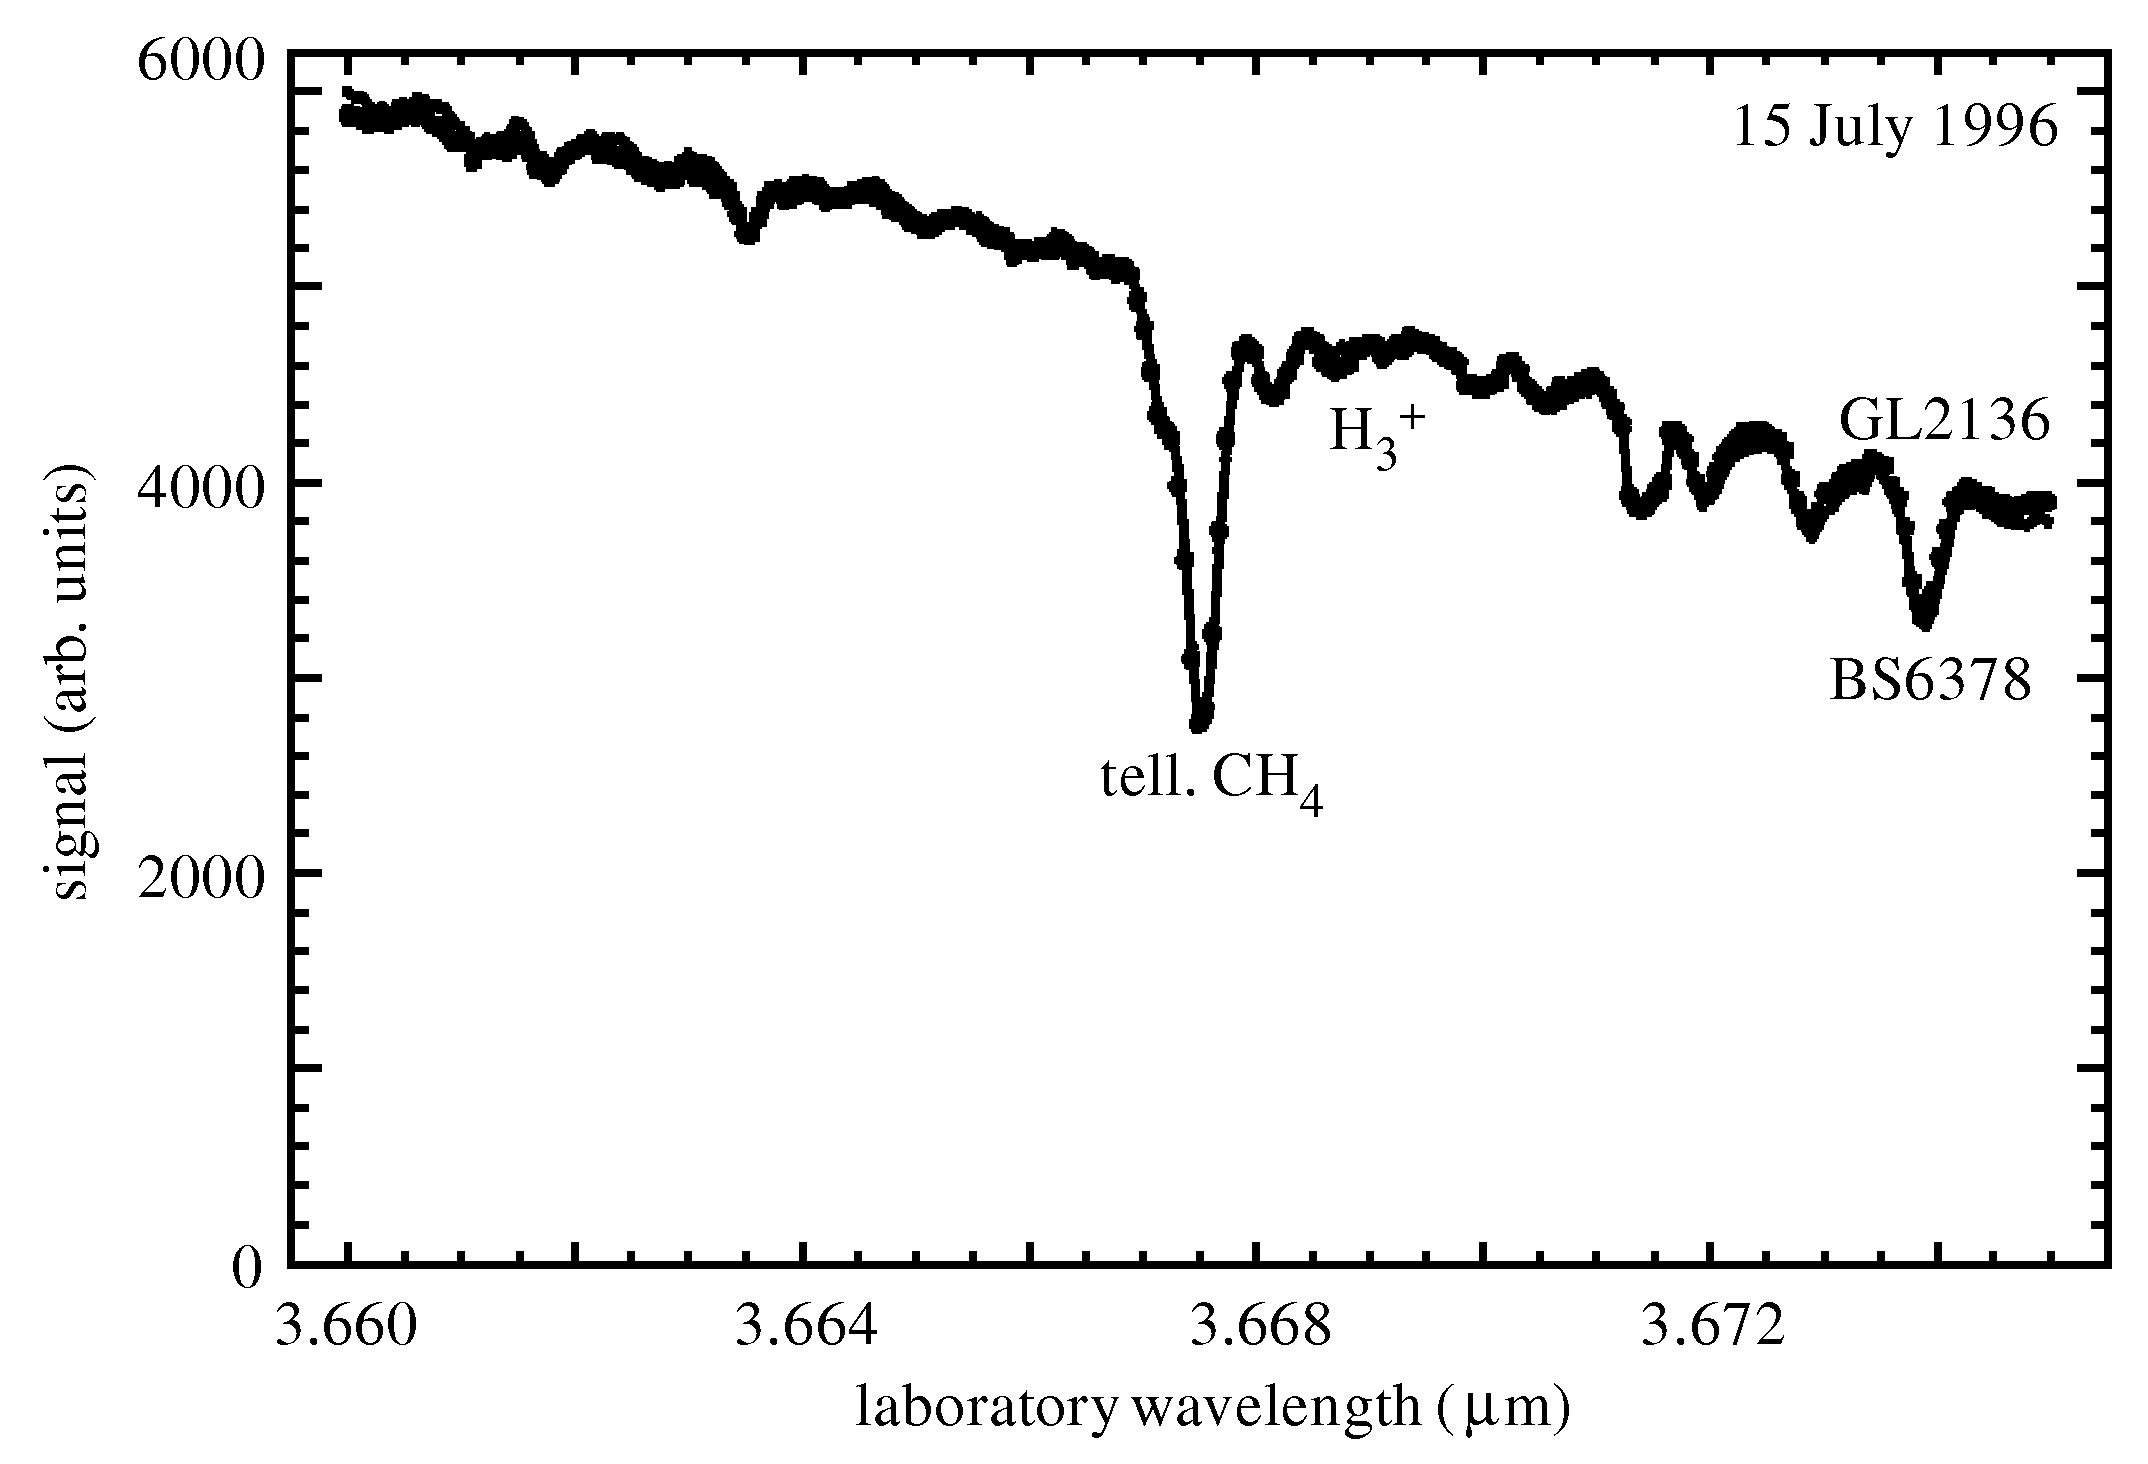
\includegraphics[width=\textwidth,height=!]{./B/h3_rawspec.jpg}
\end{center}

\end{frame} \begin{frame}\frametitle{}
\begin{center}
  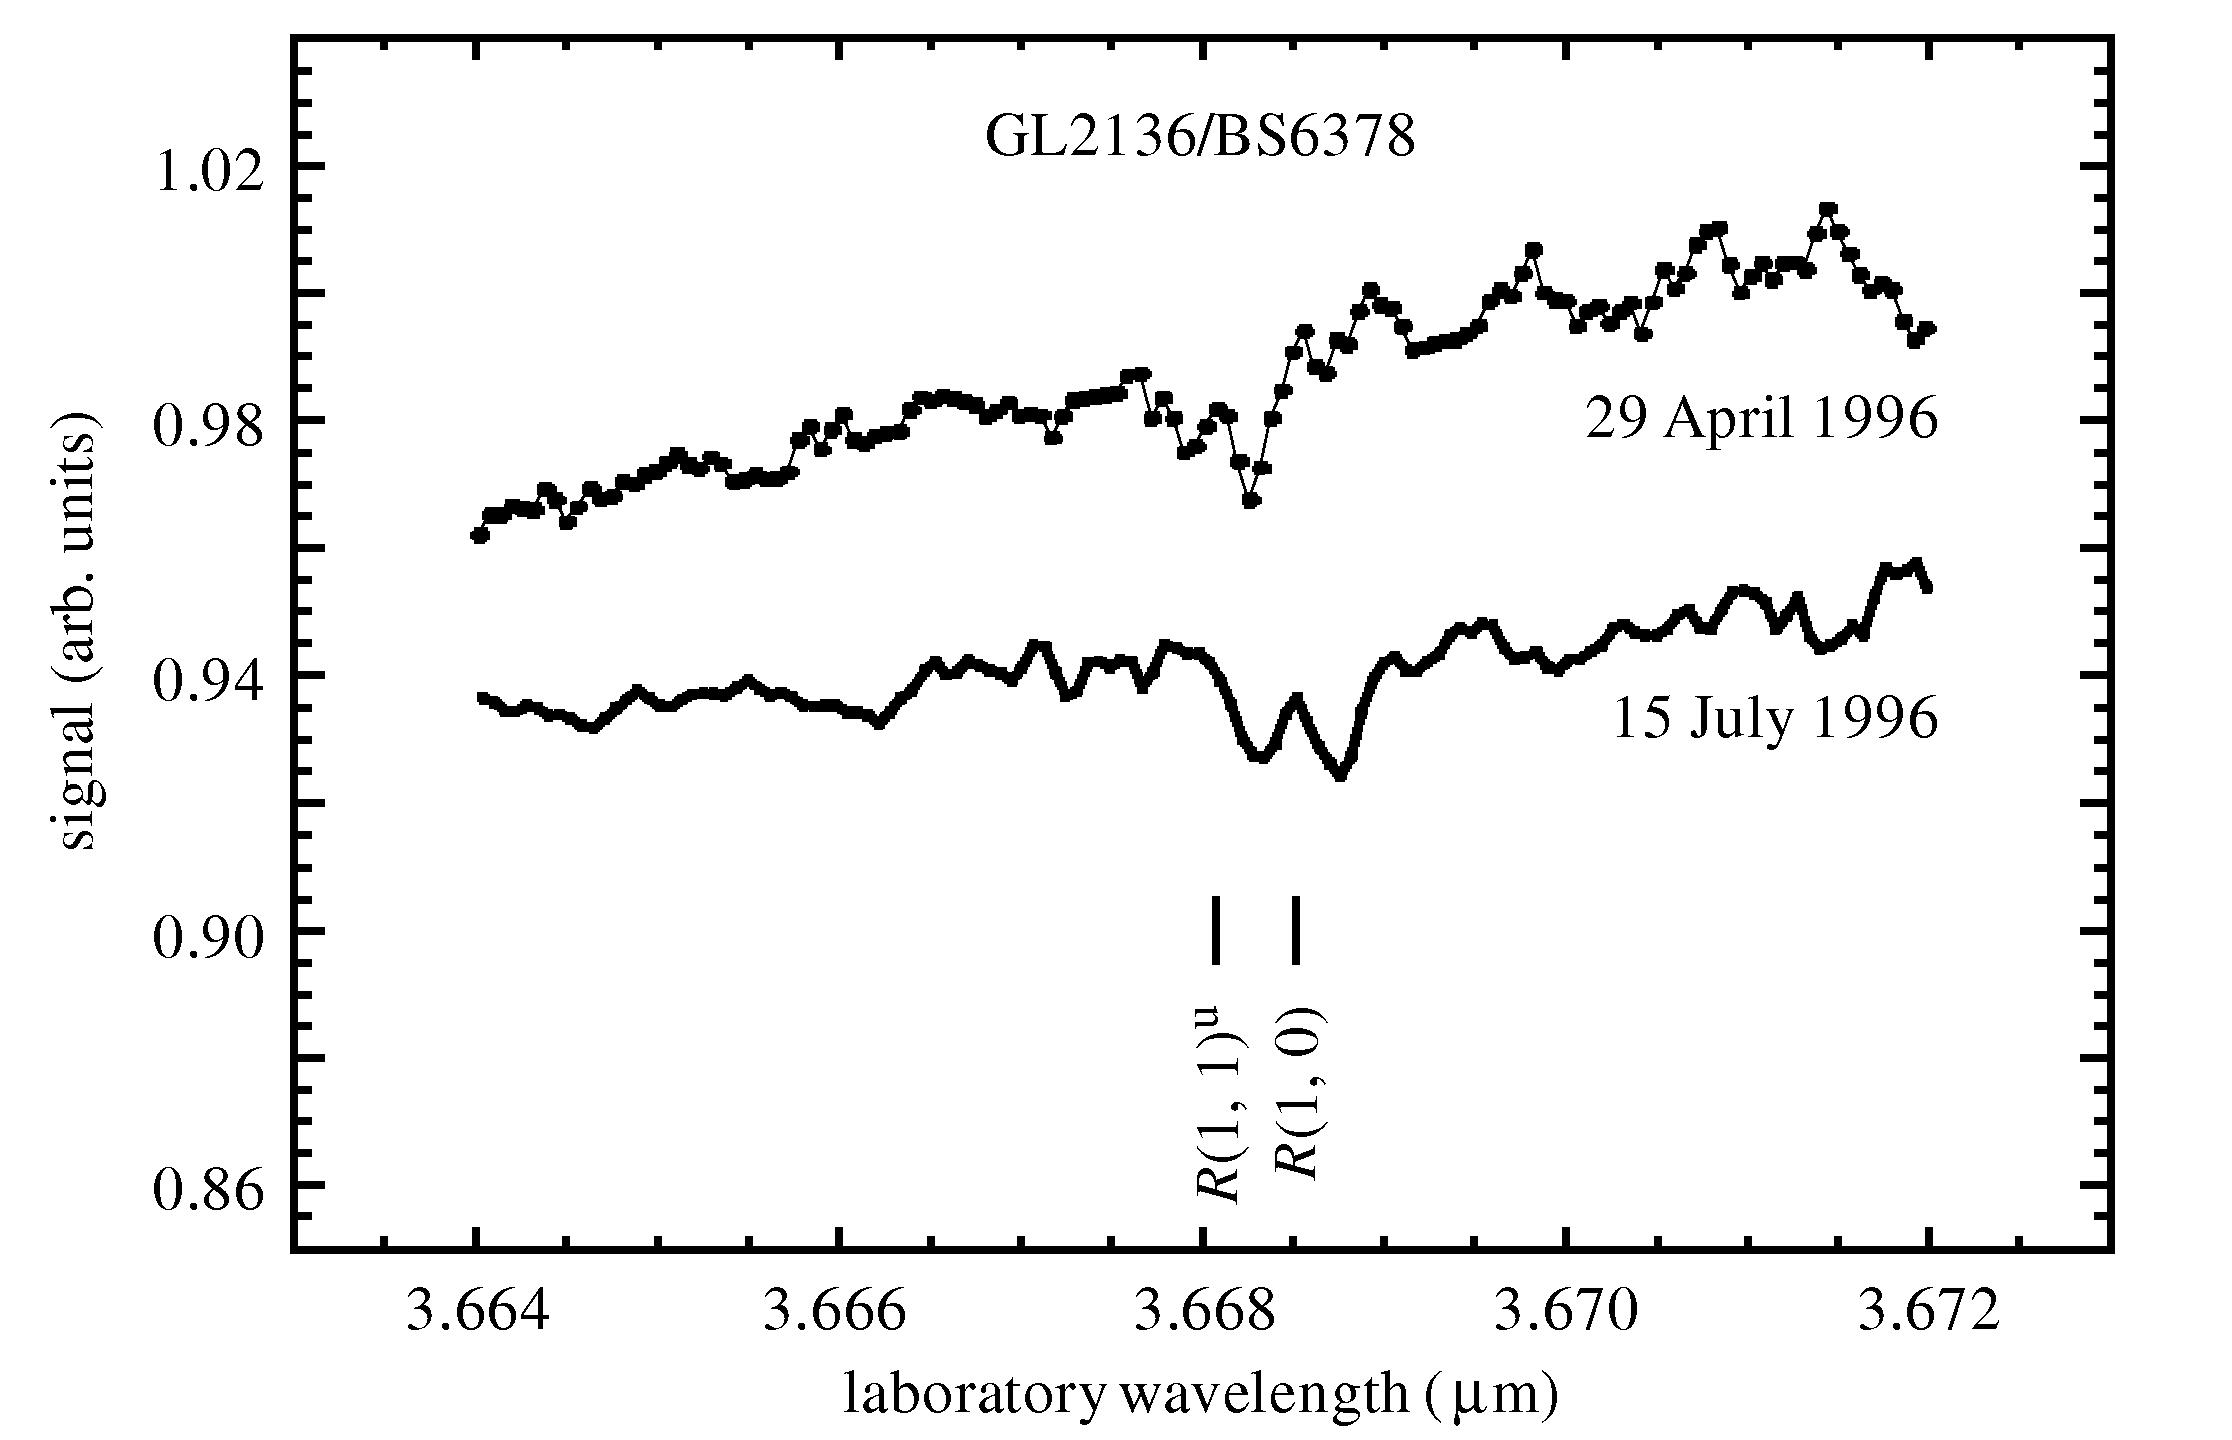
\includegraphics[width=\textwidth,height=!]{./B/h3_discspec.jpg}
\end{center}

\end{frame} \begin{frame}\frametitle{}
\begin{center}
  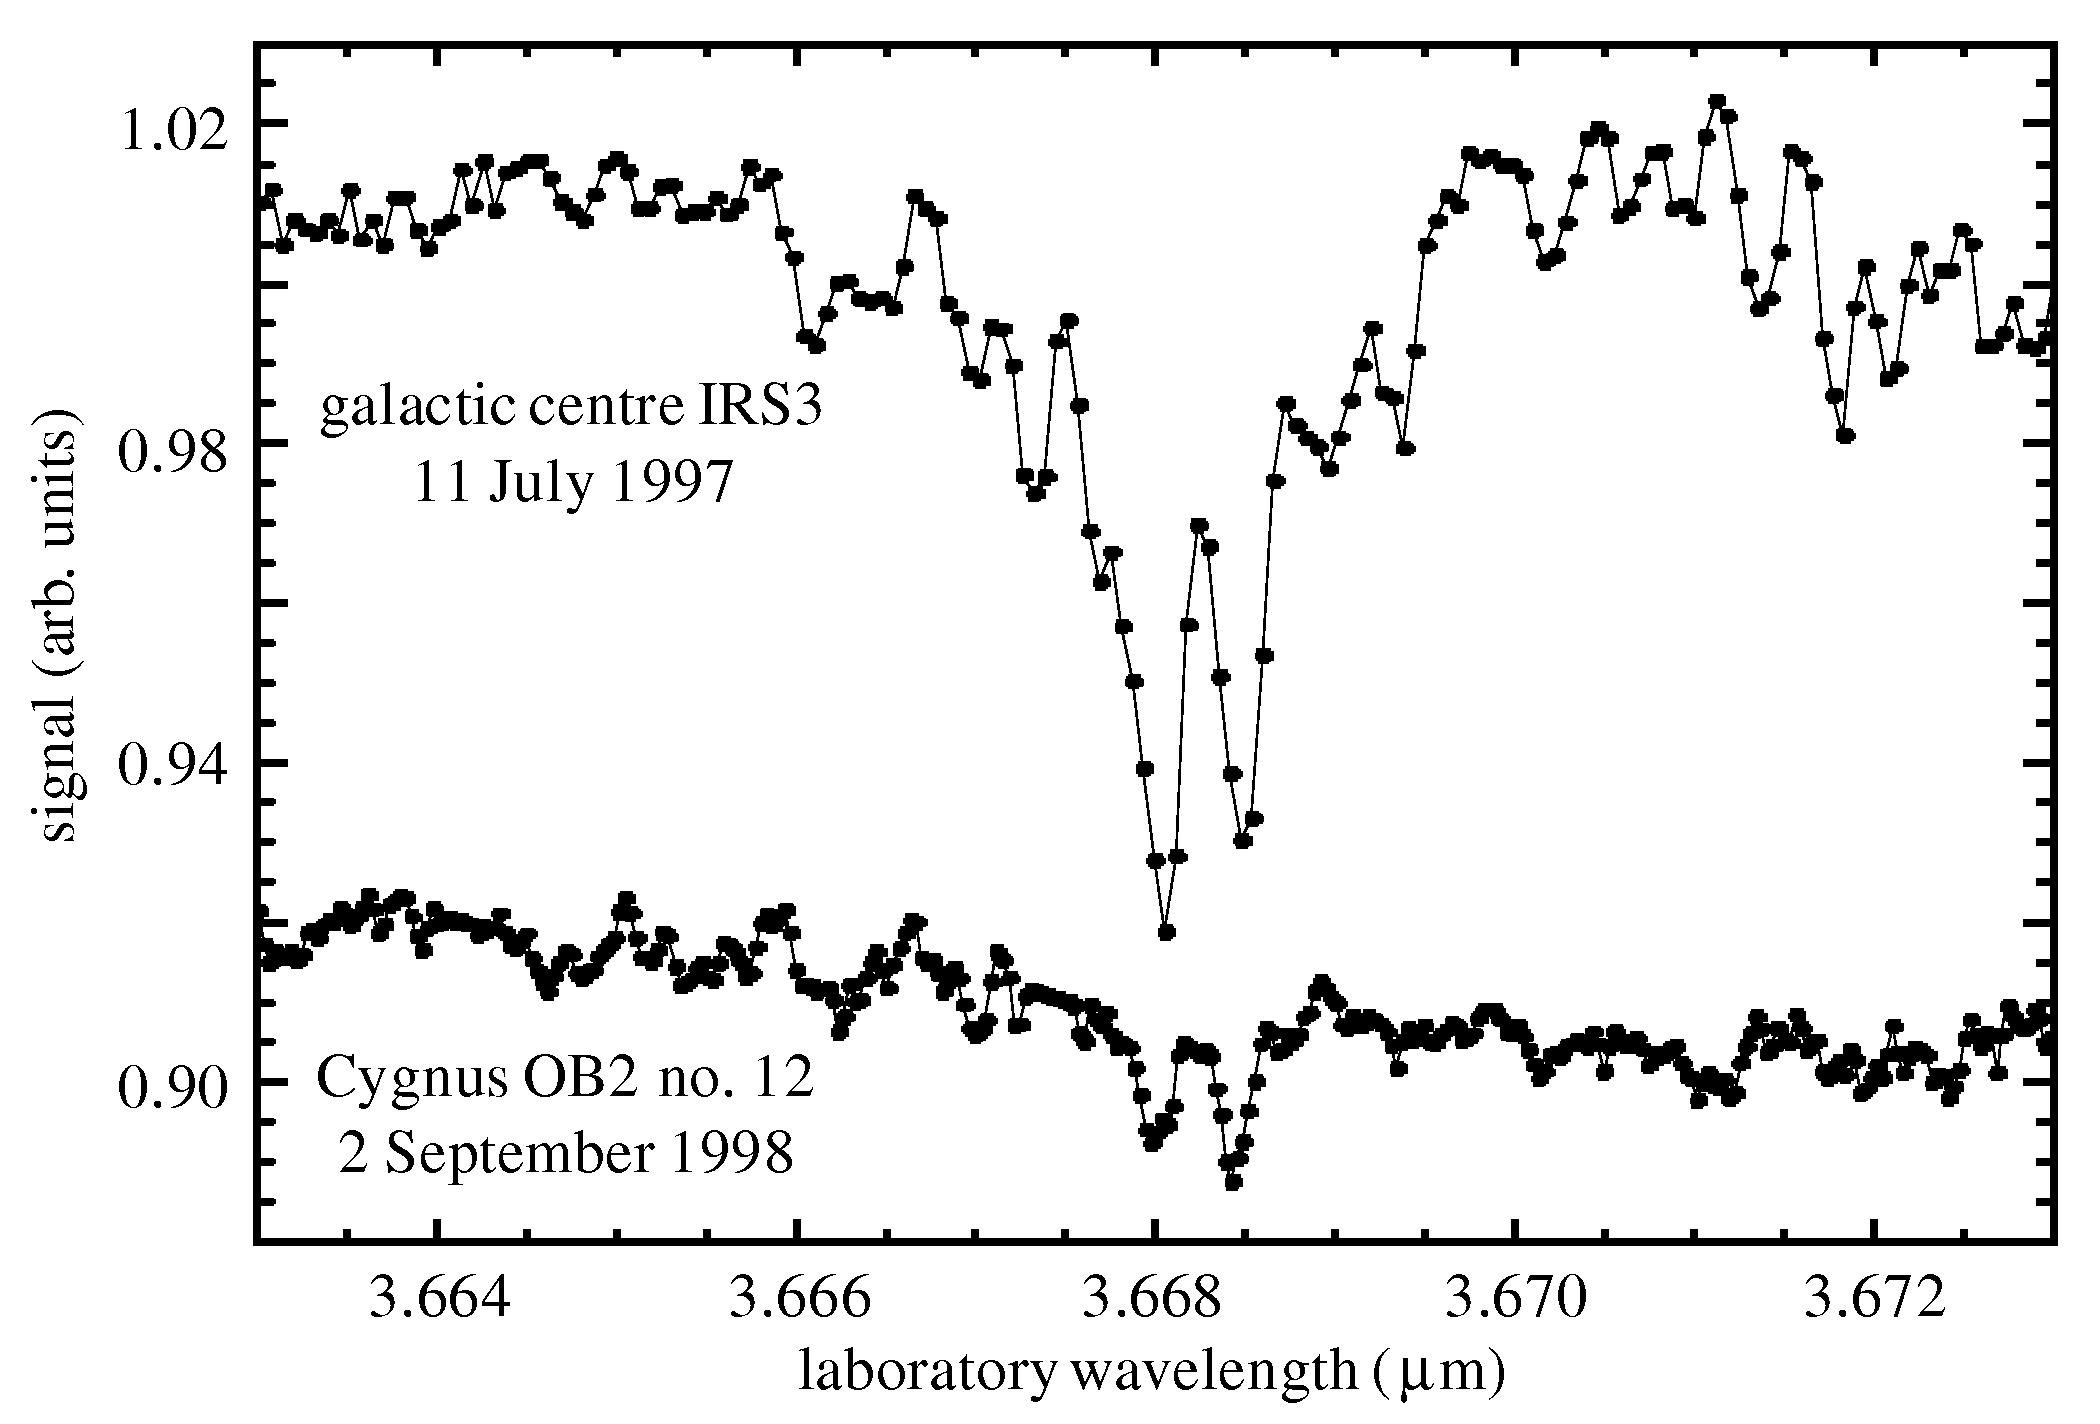
\includegraphics[width=\textwidth,height=!]{./B/h3_other.jpg}
\end{center}


\end{frame}

\subsection{Chemical fractionation}

 \begin{frame}\frametitle{ Chemical fractionation: CO}


The reaction \[ ^{13}\mathrm{C}^{+} + ~^{12}\mathrm{CO}
\overset{k_1}{\underset{k_2}{\rightleftharpoons}} ~^{12}\mathrm{C}^{+}
+ ~^{13}\mathrm{CO} + \Delta E, \]is slightly exothermic: $\Delta E /
k = 35$~K. Consequently, at low temperatures ( $\lesssim 35$~K), the
isotopic ratio $^{12}$C/$^{13}$C is different in CO than in the rest
of the {\sc ism} - there is fractionation in the C isotopes.

\end{frame} \begin{frame}\frametitle{ Chemical fractionation: theory}


At constant $P$ and $T$, minimizing the free energy $G$ gives $
\sum_i \nu_i \mu_i = 0$, and allows relating the concentration of each
species involved in the reaction. For reactions in the gas phase, we
can use the chemical potential of ideal gases,
$ \mu_i = k T \ln \left[ n_i / {\mathcal{Z}_i(T)} \right]$, 
with the partition function  \[\mathcal{Z}_i(T) = \frac{h}{\sqrt{2 \pi m_i
~k\,T}} \sum_a g^a_i e^{-\xi_a/kT}, \] where the energies associated
with the internal degrees of freedom are referred to the ground
state. We get the law of mass-action (e.g. Shu~I, 7), \[
\prod_i n_i^{\nu_i} = \prod_i \mathcal{Z}_i^{\nu_i}   .\]


\end{frame} \begin{frame}\frametitle{Application to CO} 

For CO fractionation,
\[  \frac{n(^{13}\mathrm{C}^{+}) ~n(^{12}\mathrm{CO})}{ n(^{12}\mathrm{C}^{+})
  ~n(^{13}\mathrm{CO})} = e^ {- \frac{1}{kT} \left(
  \xi(^{12}\mathrm{CO}) - \xi(^{13}\mathrm{CO} ) \right)} = \exp\left(
  -\frac{\Delta E}{kT} \right) , \] where the ground state energy is  $\xi(^{12}\mathrm{CO})$.

For CO, the rates of reactions in both directions are fast, $k_1 = k_2
= 2~10^{-10}~$cm$^3$~s$^{-1}$, and for cold clouds with  $n(H_2)
\approx 10^{4}~$cm$^3$ and $n_\mathrm{CO}/n_\mathrm{H_2} \approx
10^{-4}$, the relaxation time is $\tau_\mathrm{frac} \lesssim
1000~$yr. Thus CO is enriched in $^{13}$C, at the expense of the rest
of the molecules.

The work function of a dust grain for the adsorption of CO is
$\Delta\,H\sim$900~K, and for $T \lesssim 900~$K the probability of
adsorption for grain-CO collisions is 1. Besides the vapor pressure of
CO is very high compared to typical {\sc ism} pressures (Leger, 1983,
A\&A, 123, 271). CO is expected to be substantially (of order 50\%)
condensed onto icy CO mantles on the surface of grains (Whittet et
al. 1985, MNRAS, 216, 45).



\end{frame} \begin{frame}\frametitle{}

\begin{wrapfigure}[8]{l}{0.49\textwidth}
    \vspace{-0.5cm}
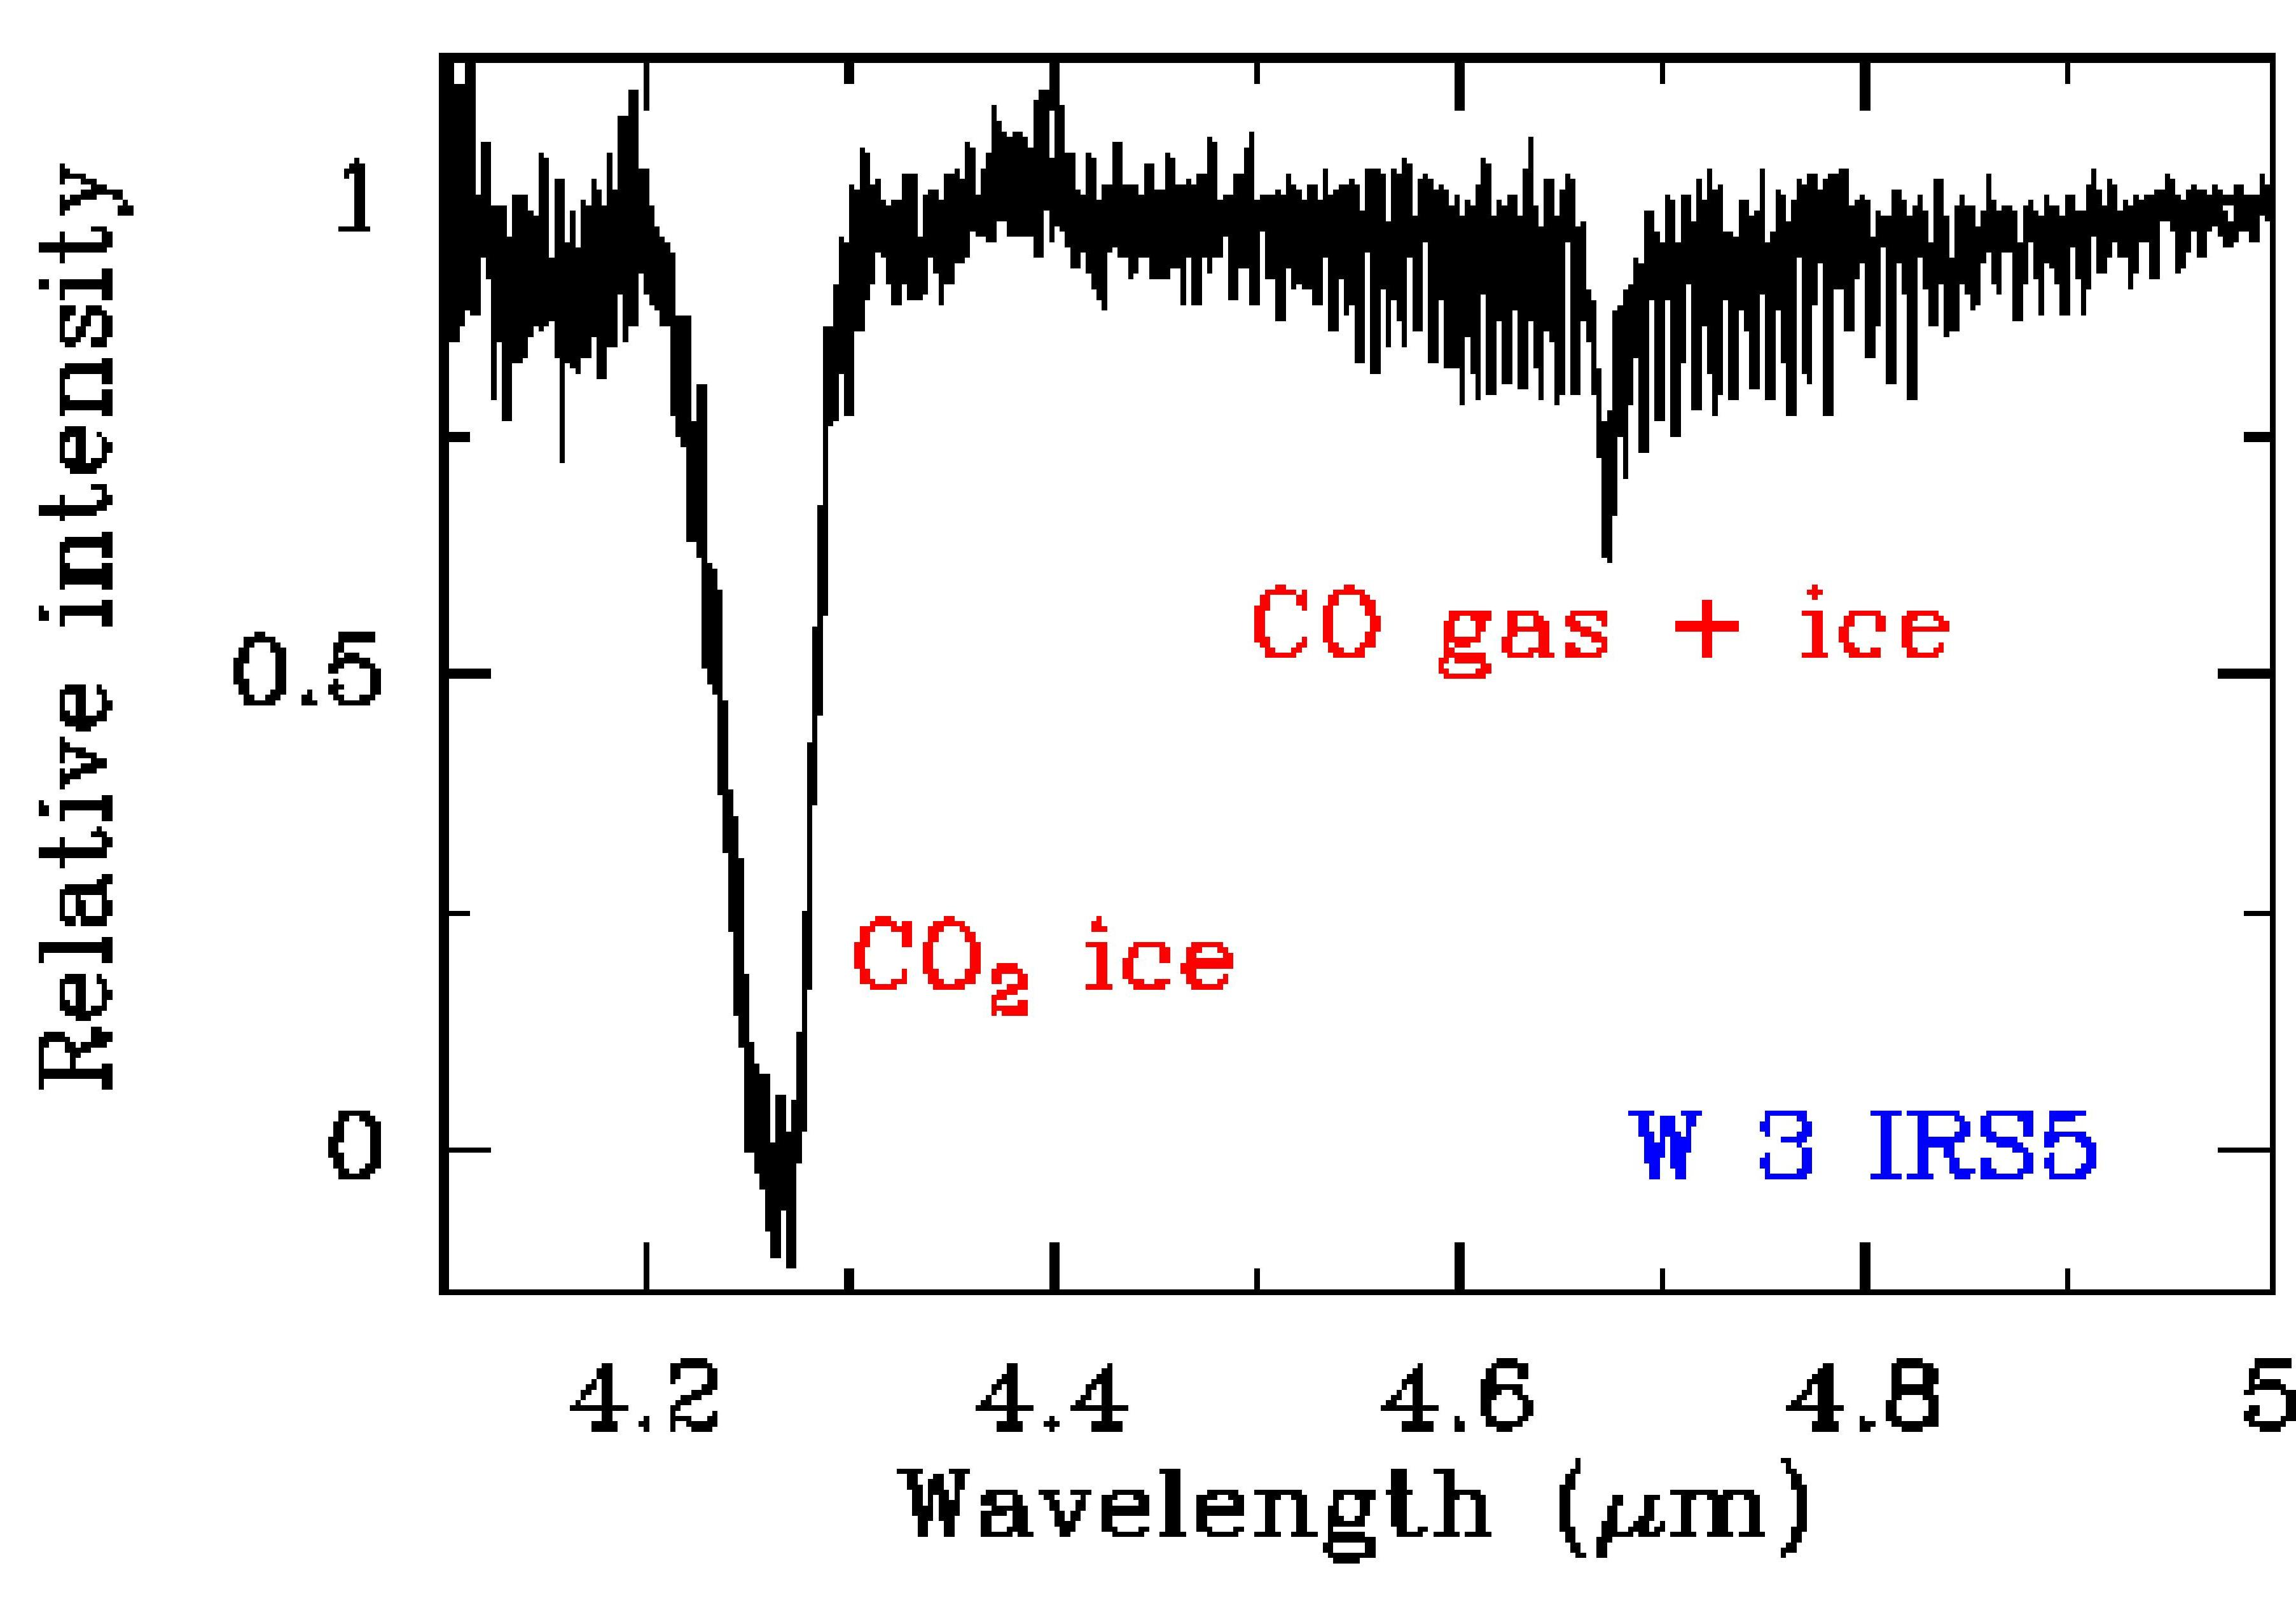
\includegraphics[width=0.49\textwidth,height=!]{./B/vandishoeck_fig4_straight.jpg}
\end{wrapfigure}  \vspace{0.1cm}  We see that the isotopic ratio
$^{12}$C/$^{13}$C will be different in the dust than in the gas phase.
Additionally the C ratio in any given molecule of the gas phase will
depend on the details of the synthesis reactions. The position taken
by CO in relation to C$^+$ will determine the C ratio in the product
molecule. This result bears on the study of the chemical evolution of
galaxies, as well as on studies of molecular cloud structure based on
the optically thin isotopes.

Chemical fractionation competes with the process of selective
photodissociation.  $^{13}$CO is dissociated by interstellar UV
radiation, penetrating to deeper lying layers in the clouds than for
the main isotope, $^{12}$CO.

\end{frame}



